\documentclass{beamer}
\usepackage{hyperref}
\usepackage{graphicx}
\usepackage{caption}
\usepackage{makeidx}
\usetheme{metropolis}

% my Colors
\definecolor{HS-Blue}{HTML}{185363}

% Change the primary color
\setbeamercolor{palette primary}{bg=blue, fg=white}
\setbeamercolor{frametitle}{bg=HS-Blue}

% Optional: Customize other colors
\setbeamercolor{title separator}{fg=HS-Blue}
\setbeamercolor{progress bar}{fg=HS-Blue}
\setbeamercolor{block title}{bg=blue!70, fg=white}
\setbeamercolor{block body}{bg=blue!20, fg=black}

\title{Erkennung von Kerben in medizinischen Stents mit Hilfe von neuronalen Netzwerken}
\subtitle{\small Notch detection on medical stents using neural networks}
\author{Yves Seburger}
\date{Kaiserslautern, der 10. Juli 2024}
\institute{Hochschule Kaiserslautern\newline
Schoenstr. 11\newline
67659 Kaiserslautern}
\titlegraphic{\hfill
\includegraphics[width=2cm]{Bilder/HSKLLogo - black font.png}}

\setbeamertemplate{frametitle}
{
    \begin{beamercolorbox}[wd=\paperwidth,ht=3ex,dp=1.125ex,leftskip=0.3cm,rightskip=0.3cm]{frametitle}
        \insertframetitle
        \hfill
        \raisebox{-0.19cm}{
\includegraphics[height=0.74cm]{Bilder/HSKLLogo - white font.png}}
         
    \end{beamercolorbox}
}

\begin{document}
\frame{\titlepage}

\begin{frame}
\frametitle{Überblick}
\tableofcontents
\end{frame}

\section{Aufgabenstellung}
\begin{frame}[allowframebreaks]
\frametitle{Aufgabenstellung}
\begin{itemize}
    \item Erstellen eines neuronalen Netzwerks
    \item Erkennen von Kerben auf Stents
    \item Visualisierung der Ergebnisse
    \newline
    \begin{figure}
        \includegraphics[width=6.5cm]{Bilder/Stent.jpg}
        \caption{(Aufnahme eines Stentteils. \scriptsize{Quelle: Yves Seburger})}
    \end{figure}  
\end{itemize}
\end{frame}


\section{Erstellung der Trainingsdaten}
\begin{frame}[allowframebreaks]
\frametitle{Erstellung der Trainingsdaten}
\begin{itemize}
    \item Aufnahme von Stentbildern:
        \begin{figure}
            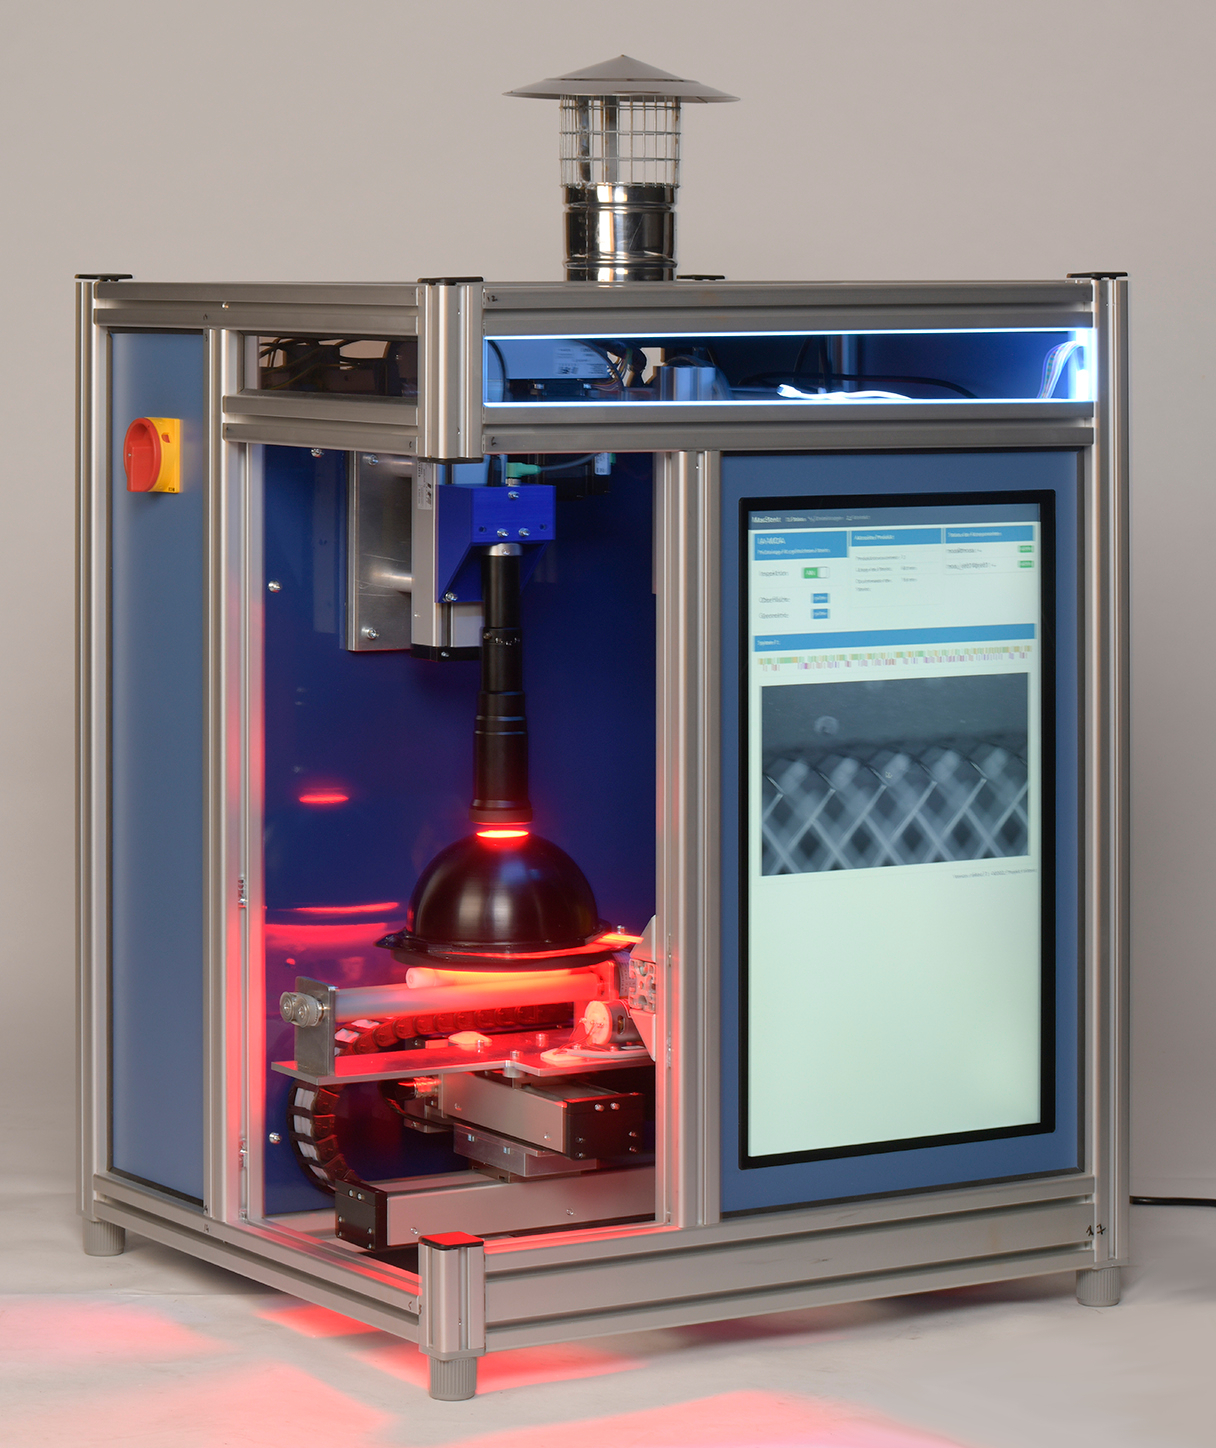
\includegraphics[height=4.75cm]{Bilder/MoA_Gesa_preversion_cut.jpg}
            \hspace{20px}
            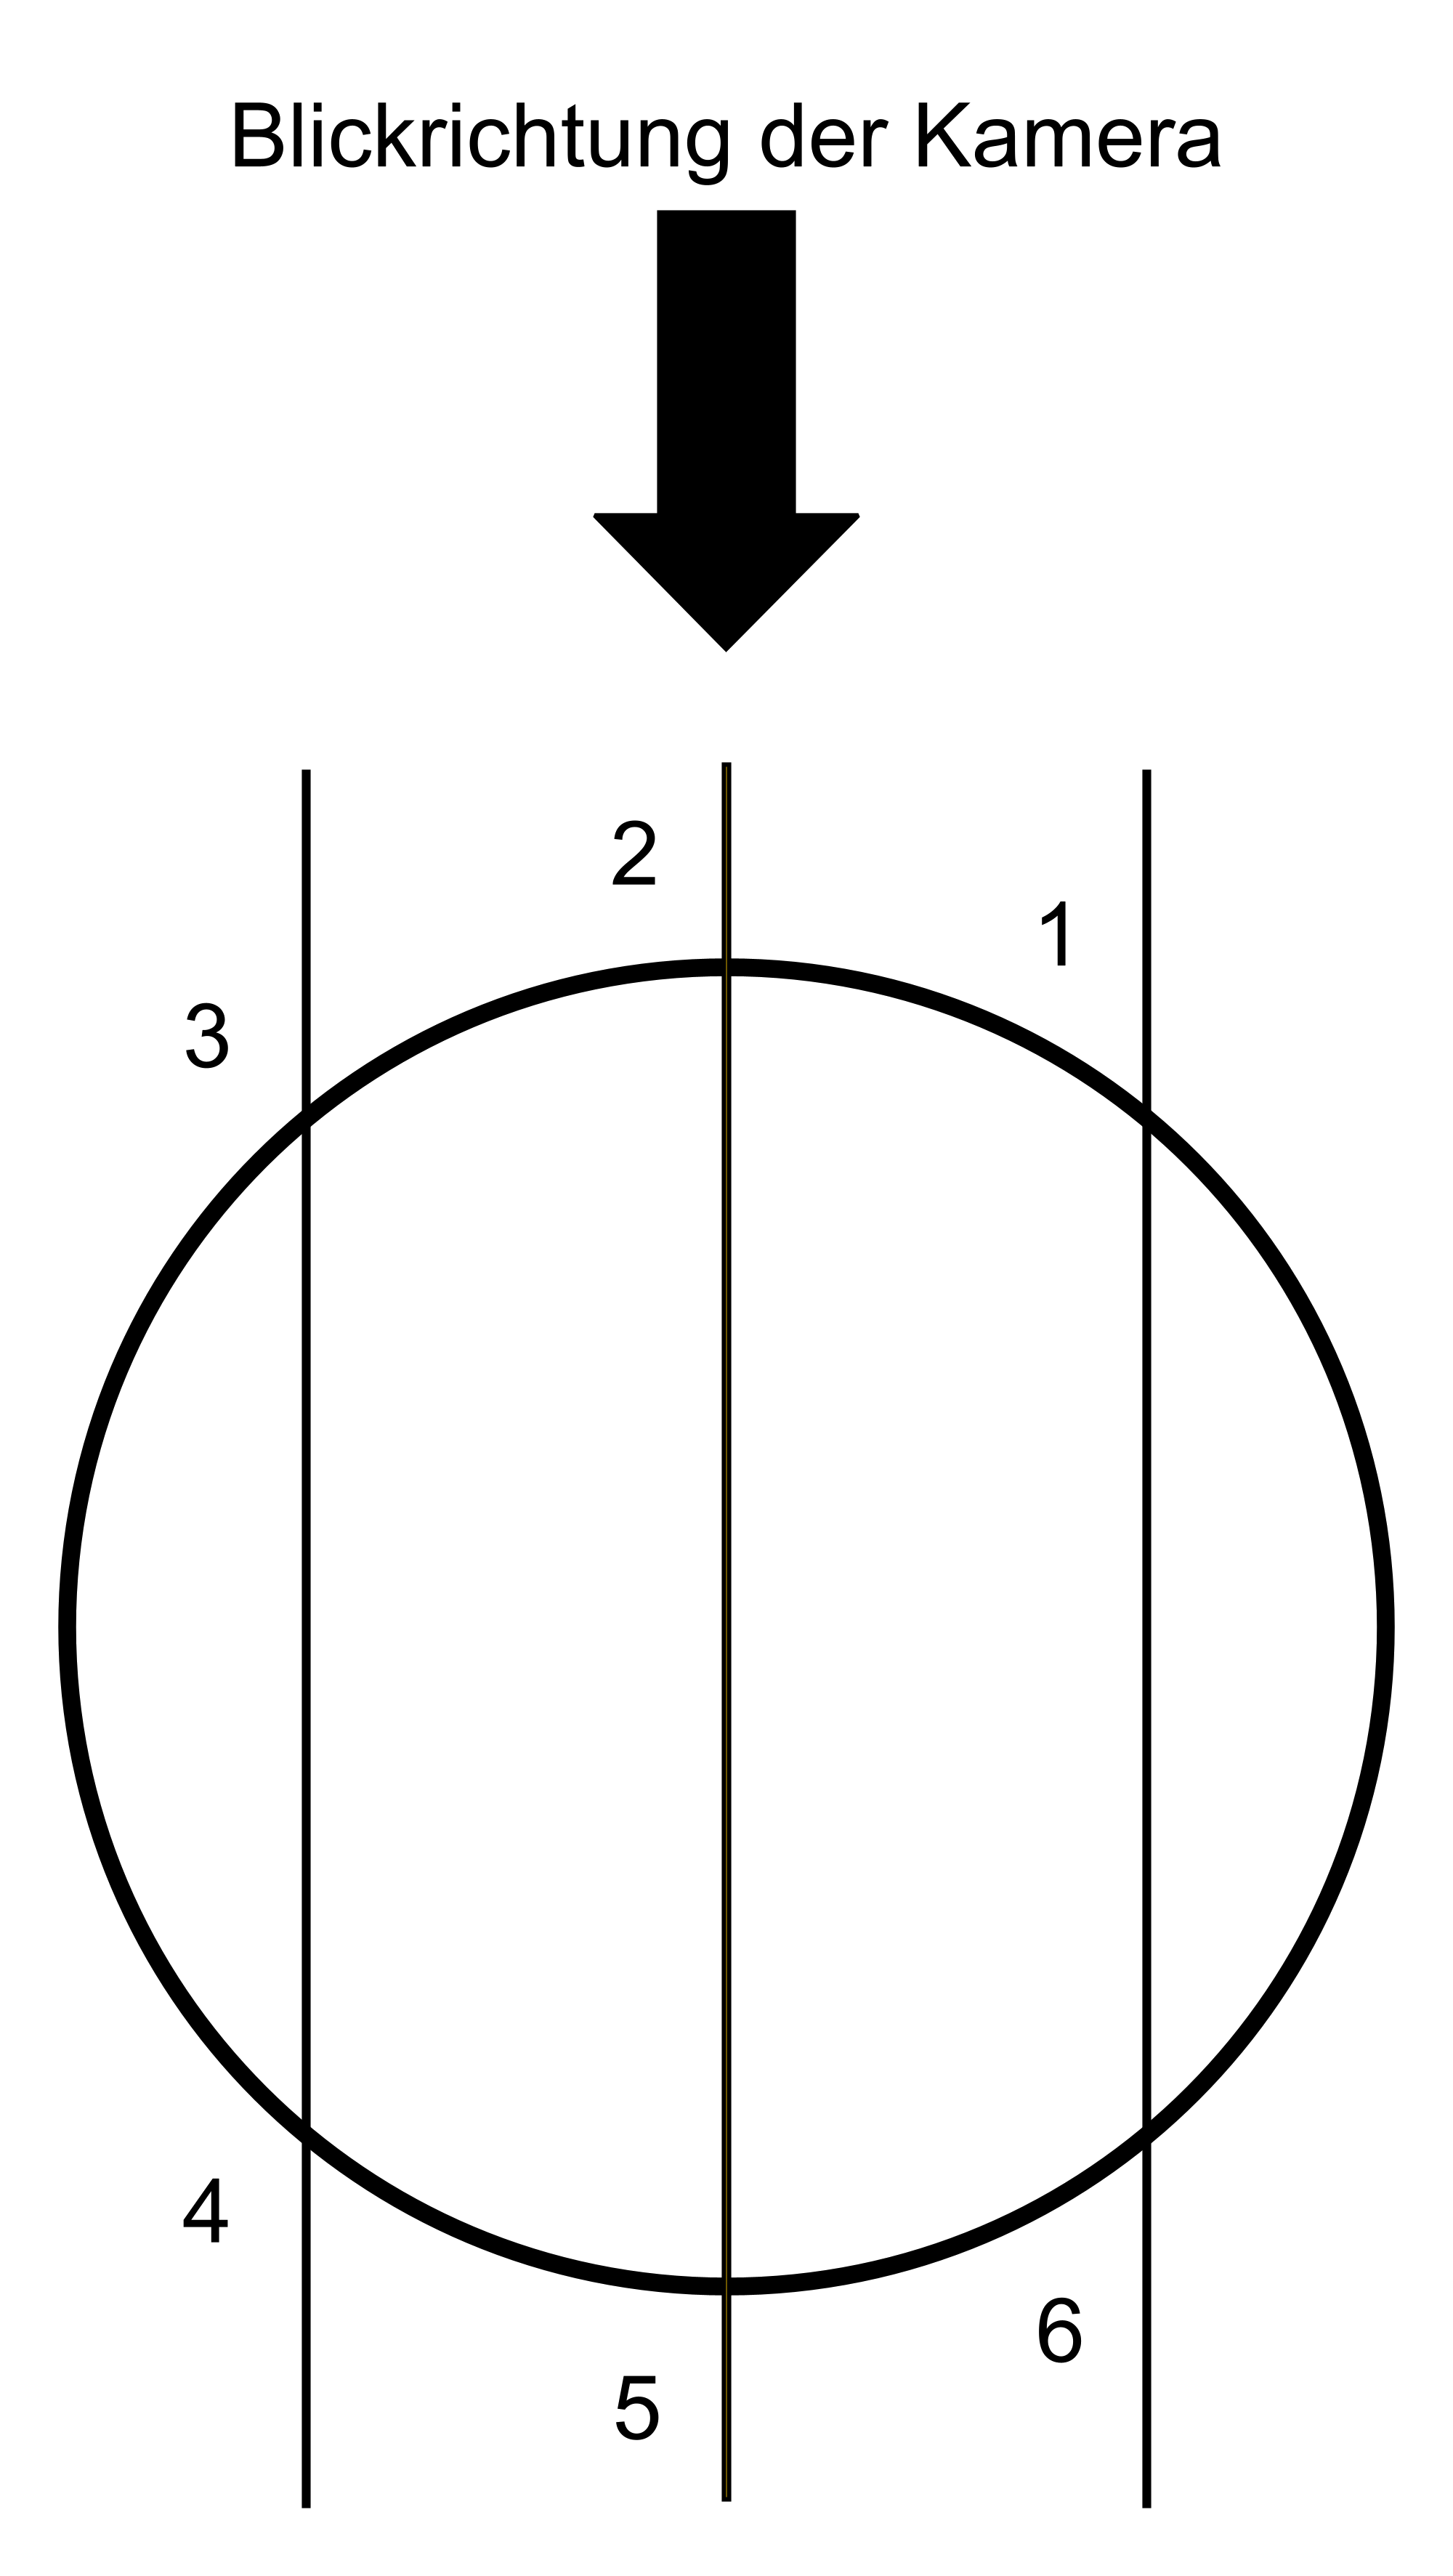
\includegraphics[height=4.75cm]{Bilder/Stentpositionen.png}
            \caption{((links) MoA Quelle: Dipl.-Ing Viktor Truderung, (rechts) Stentpositionen. \scriptsize{Quelle: Yves Seburger})}
        \end{figure}
\end{itemize}
\begin{itemize}
    \item Einschränkung von Kerbenfehlern:
        \begin{figure}
            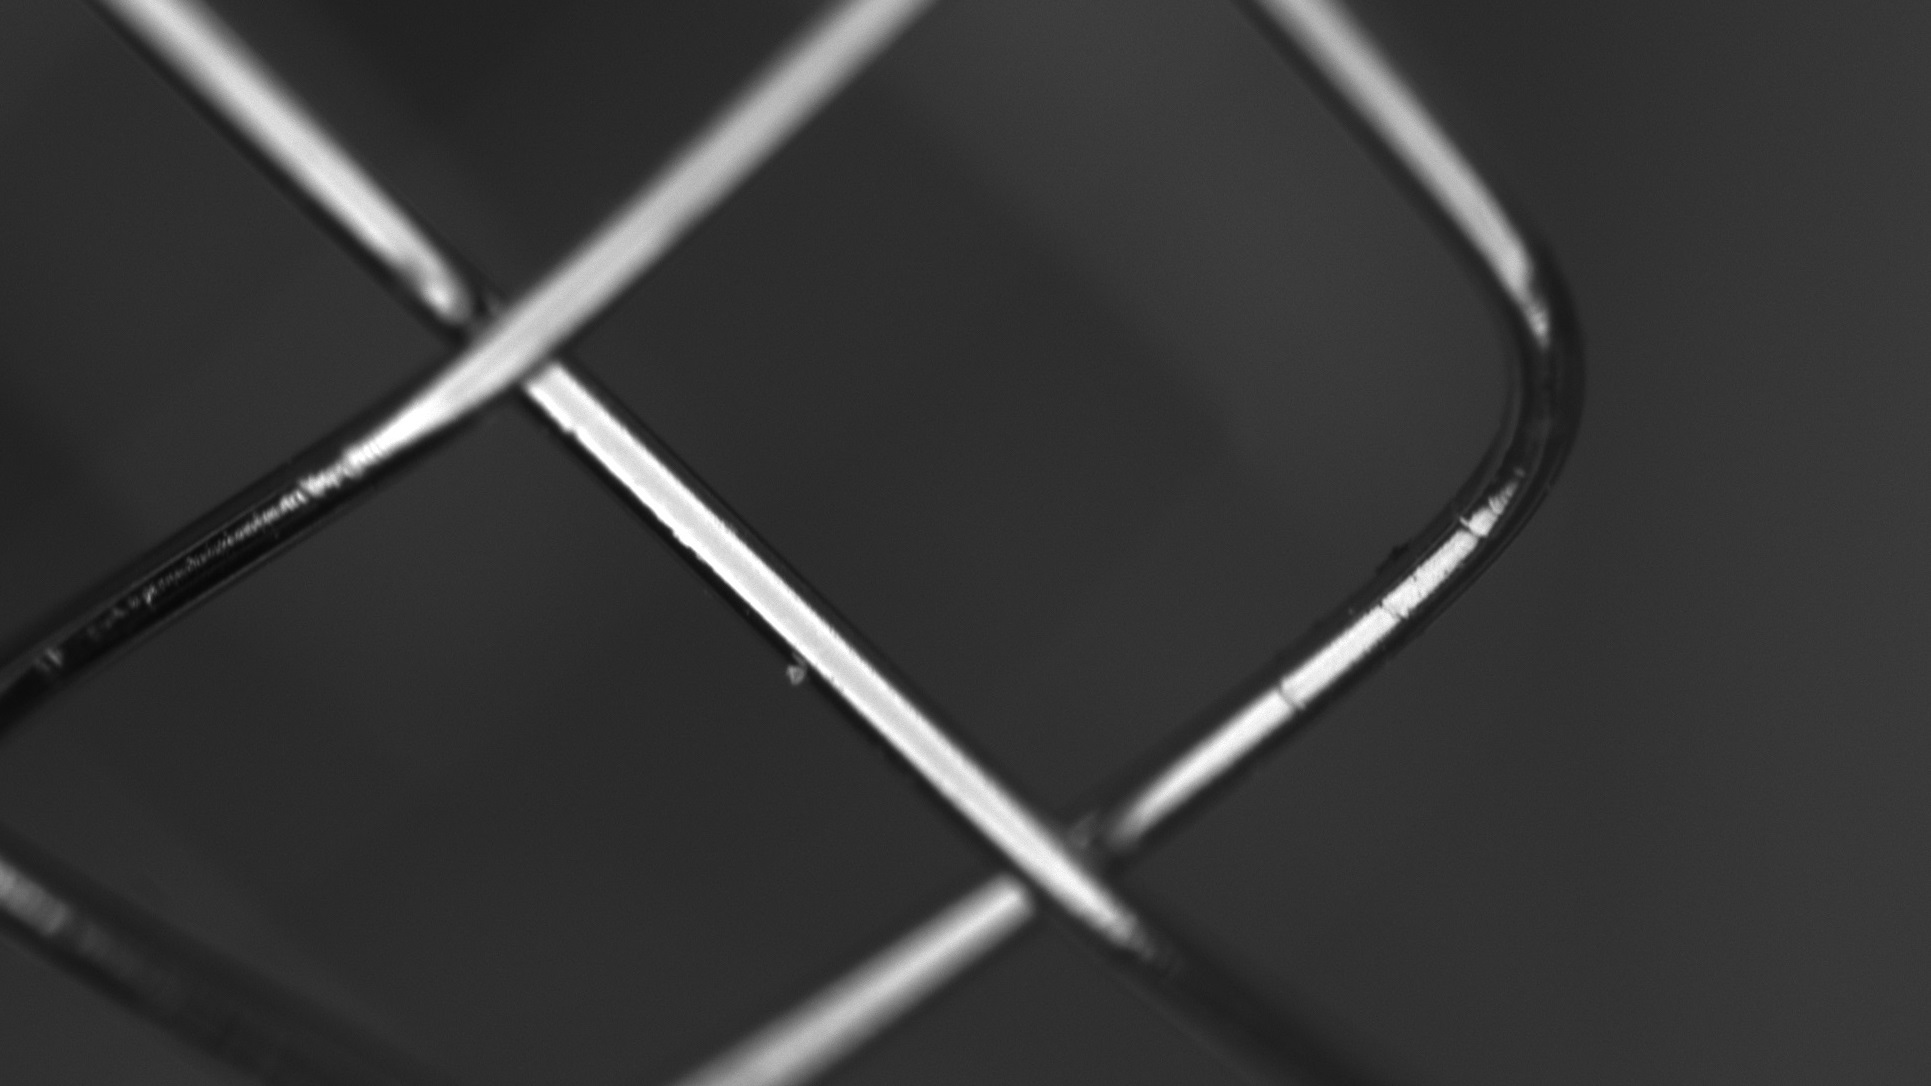
\includegraphics[width=4.5cm]{Bilder/Annotationfragen/Frage_5_crop.jpg}
            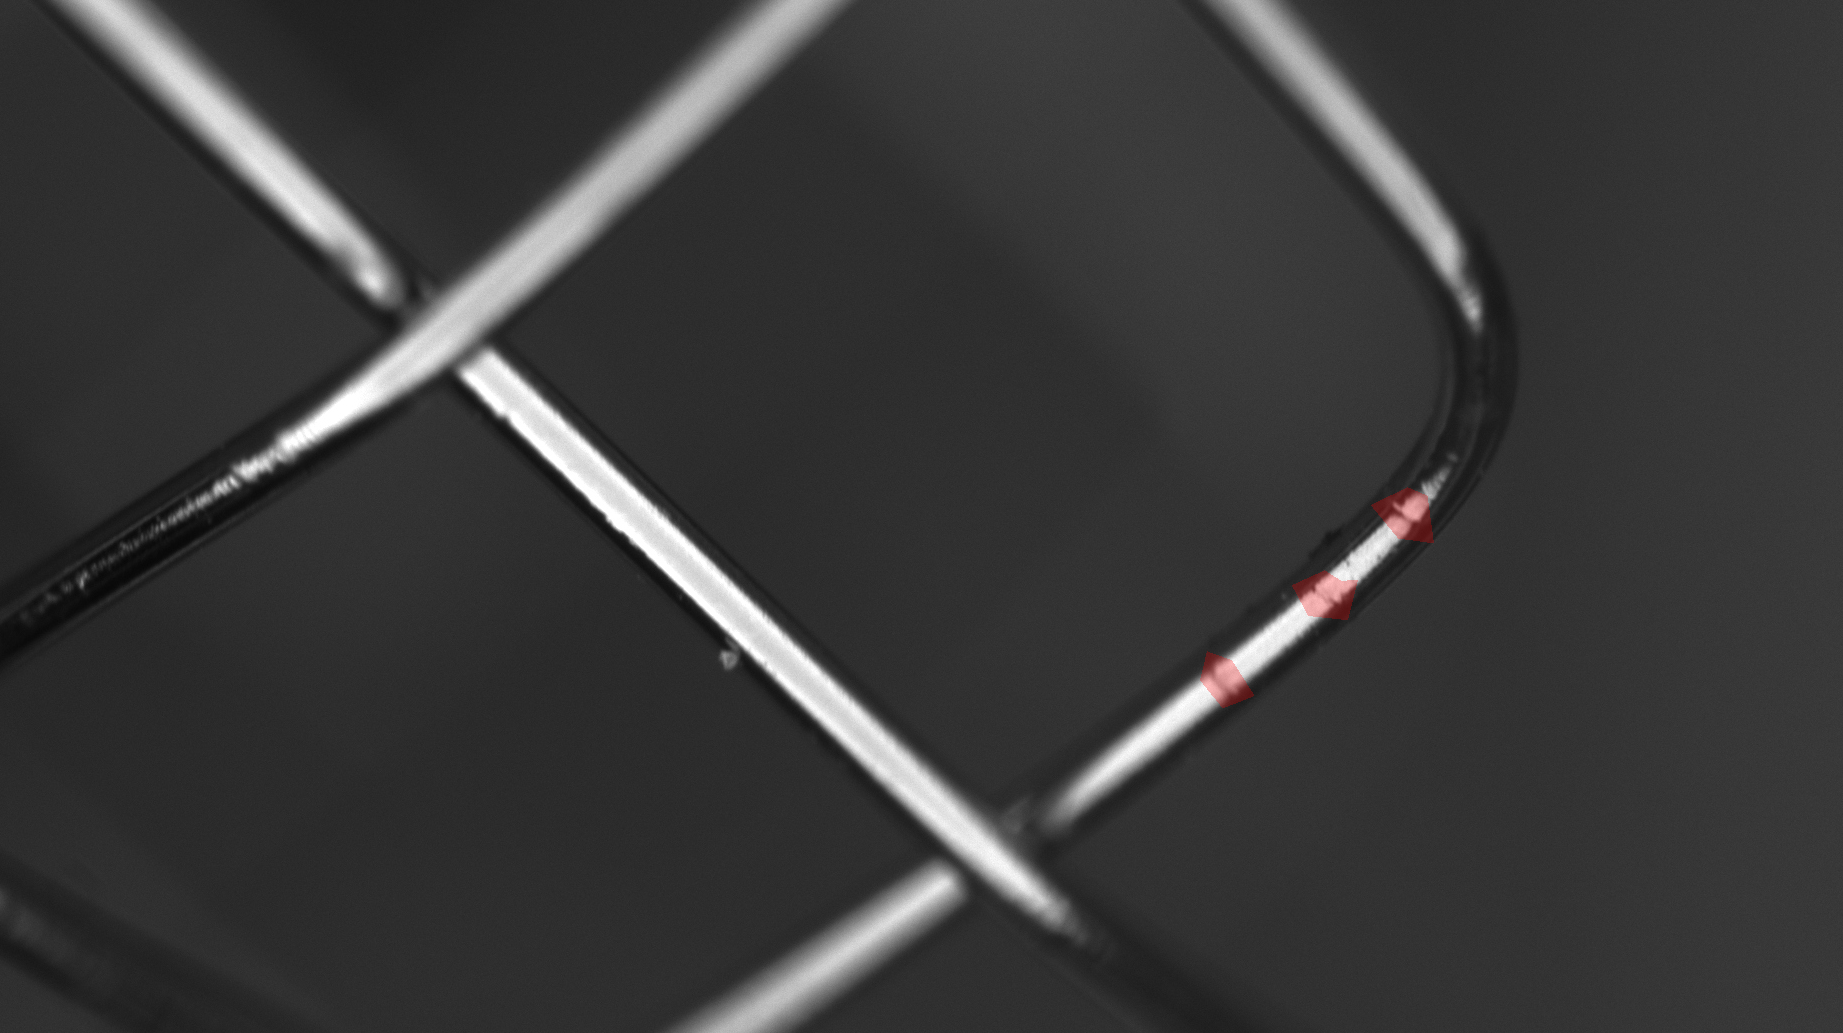
\includegraphics[width=4.5cm]{Bilder/Annotationfragen/Frage_5_anno.png}
            
\includegraphics[width=4.5cm]{Bilder/Annotationfragen/Kratzer.jpg}
            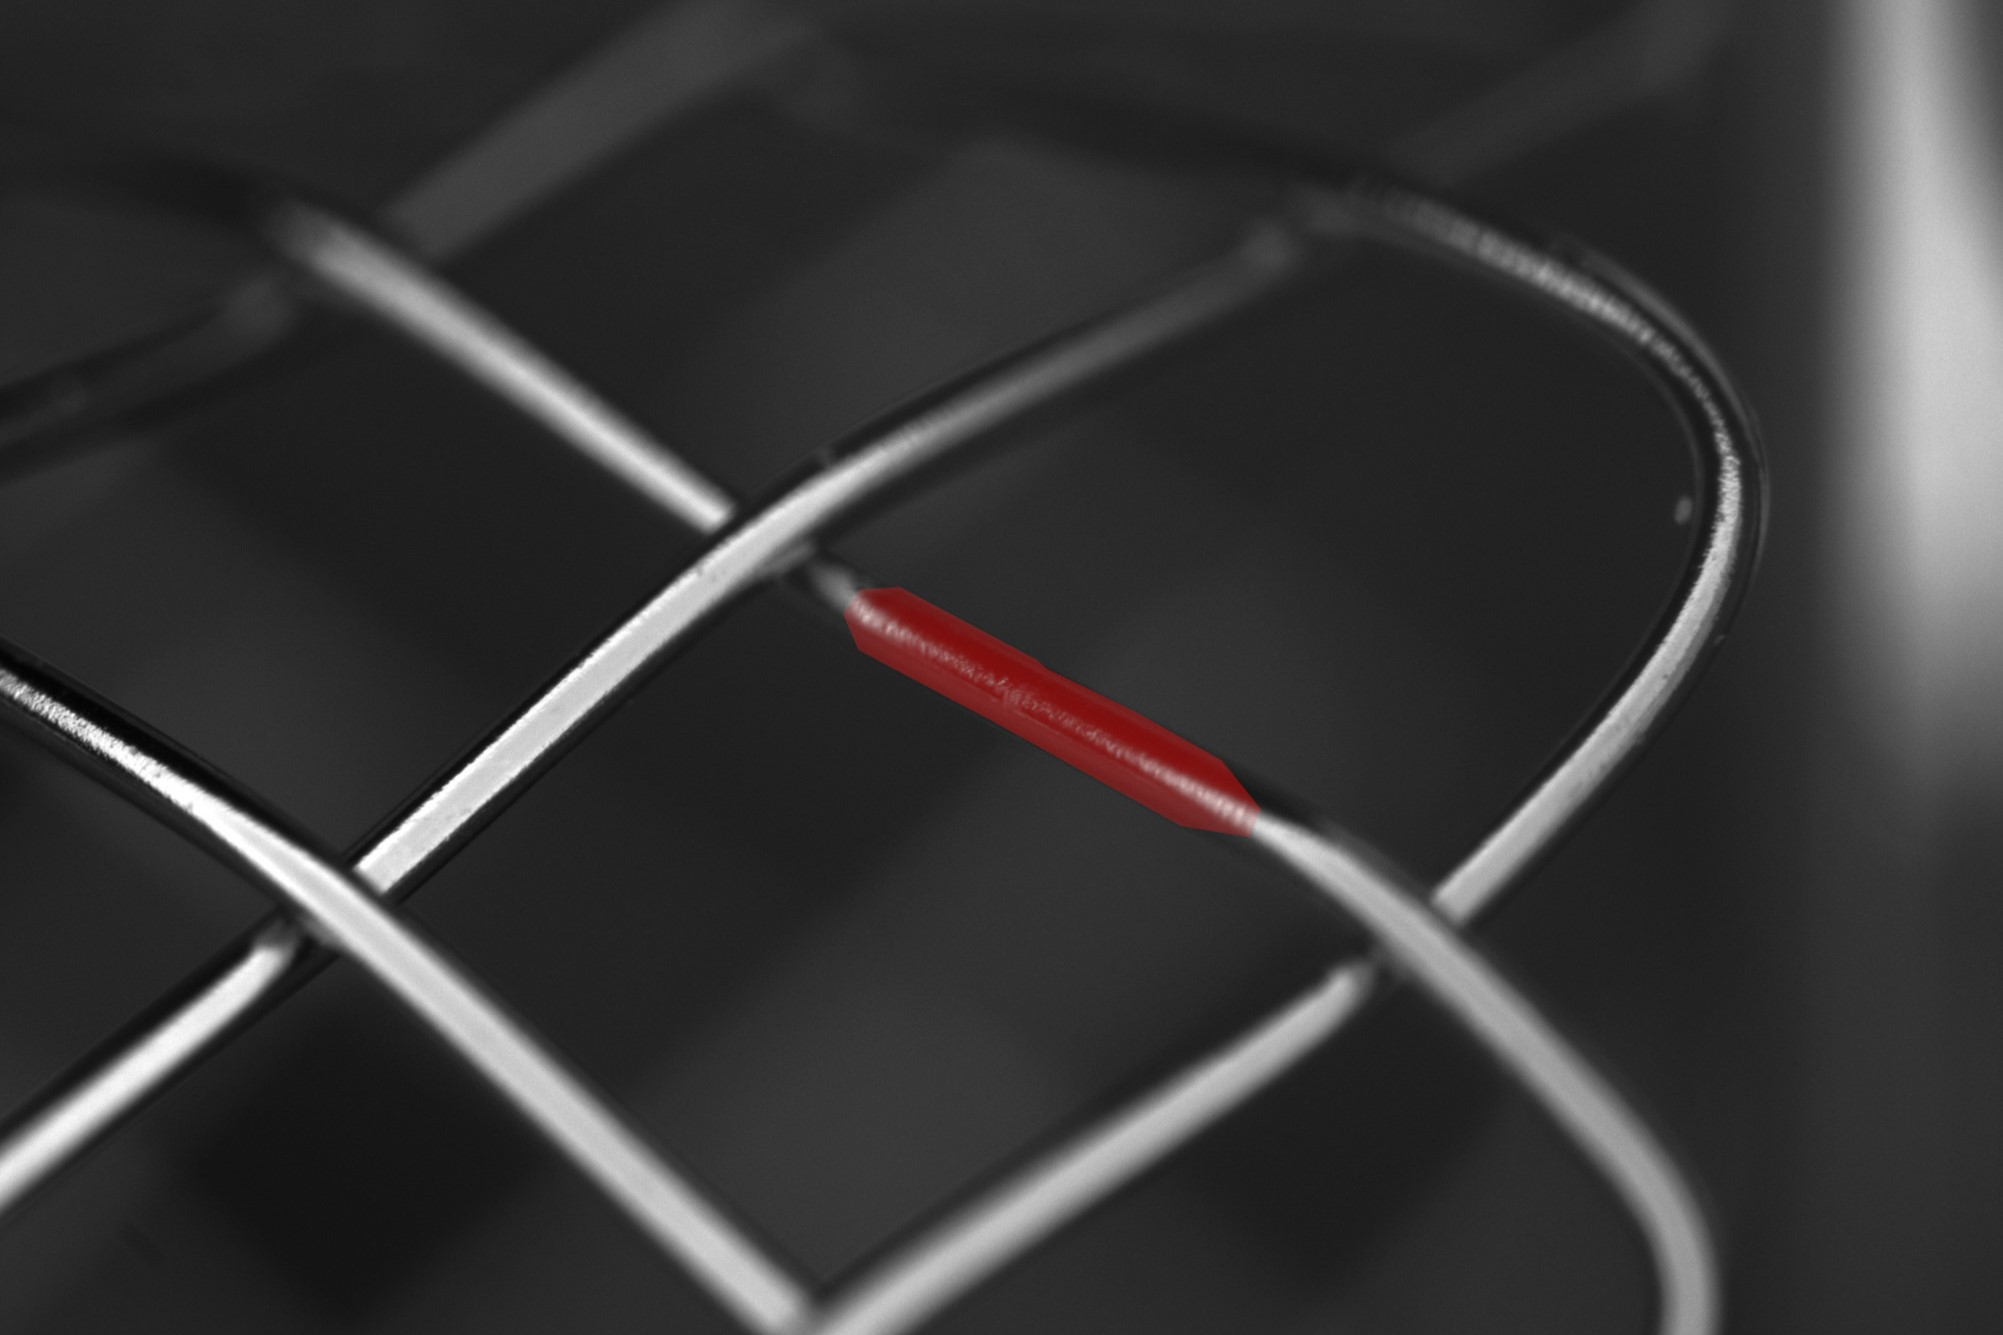
\includegraphics[width=4.5cm]{Bilder/Annotationfragen/Kratzer_anno.jpg}
            \caption{Annotierte Bilder. \scriptsize{Quelle: Yves Seburger}}
        \end{figure} 
    \item Annotation:
    \begin{figure}
        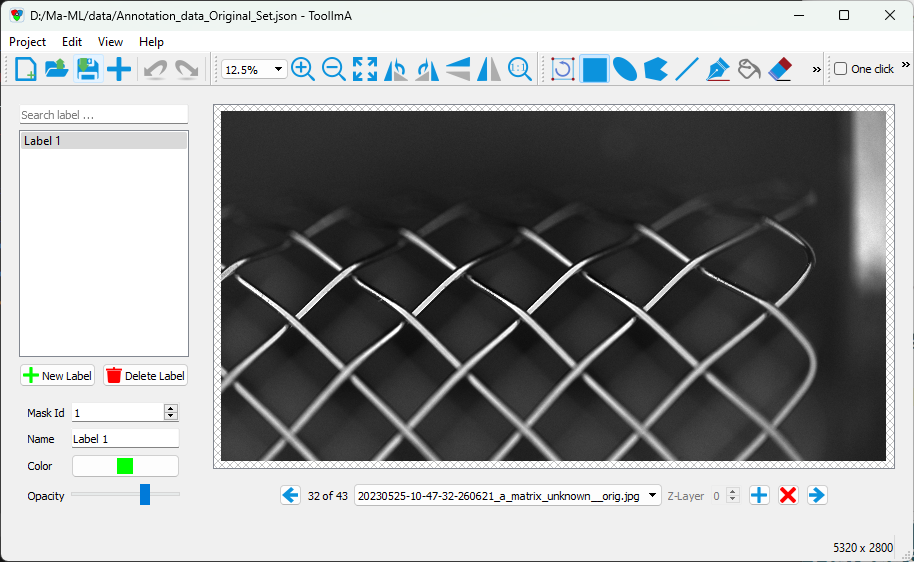
\includegraphics[width=8.7cm]{Bilder/toolima.png}
        \caption{Toolima, Software zu Annotation. \scriptsize{Quelle: Yves Seburger}}
    \end{figure} 
\end{itemize}
\end{frame}

\section{Anforderungen und Spezifikatonen zum Programm}
\begin{frame}
    \frametitle{Anforderungen und Spezifikatonen zum Programm}
    \begin{itemize}
        \item Funktionale Anforderungen:
            \begin{itemize}
                \item Einlesen von Daten
                \item Ausgabe von Ergebnissen
                \item Speichern von Gewichte
                \item Datenmenge soll erweiterbar sein
            \end{itemize}
        \item Optionale Anforderungen:
            \begin{itemize}
                \item veränderliche Hyperparameter
                \item ``einfache`` Handhabung
                \item schnelles Training ohne große Verluste
            \end{itemize}
        \item Technische Spezifikationen: 
        ML-fähige GPU (AMD (ROCm) oder Nvidia (Cuda)), 
        Python, Pytorch, numpy, etc.
    \end{itemize}
\end{frame}

\section{Herausforderungen}
\begin{frame}
\frametitle{Herausforderungen}
\begin{itemize}
    \item Anzahl der Originalbilder
    \item Fehlerannotierung:
    \begin{itemize}
        \item Kratzer sollen nicht annotiert werden
        \item Kerben ``pixelgenau'' annotieren
    \end{itemize}
    \item normaler Dice-Score:
    $Dice = \frac{2 \cdot A \cap B}{A + B}$ 
    \item Aufteilung der Originaldaten:
    \begin{itemize}
        \item 80/20-Regel
        \item verschiedene Fehlertypen
    \end{itemize}
\end{itemize}
\end{frame}

\section{Methodik}
\begin{frame}[allowframebreaks]
\frametitle{Methodik}
\begin{itemize}
    \item gewichteter Dice-Score:\\
    \begin{equation}
        \begin{split}
            Dice &= \frac{2 \cdot A \cap B}{A + B}\\
            &= \frac{2 \cdot TP}{TP + FP + FN}\\
            Dice_g &= \frac{2 \cdot TP}{TP + \alpha \cdot FP + FN}
            \,\,\,(mit\, \alpha \leq 1)
        \end{split}
    \end{equation}
    \framebreak
    \item Augmentierung:
    \begin{itemize}
        \item Spiegelung:
        \begin{figure}
            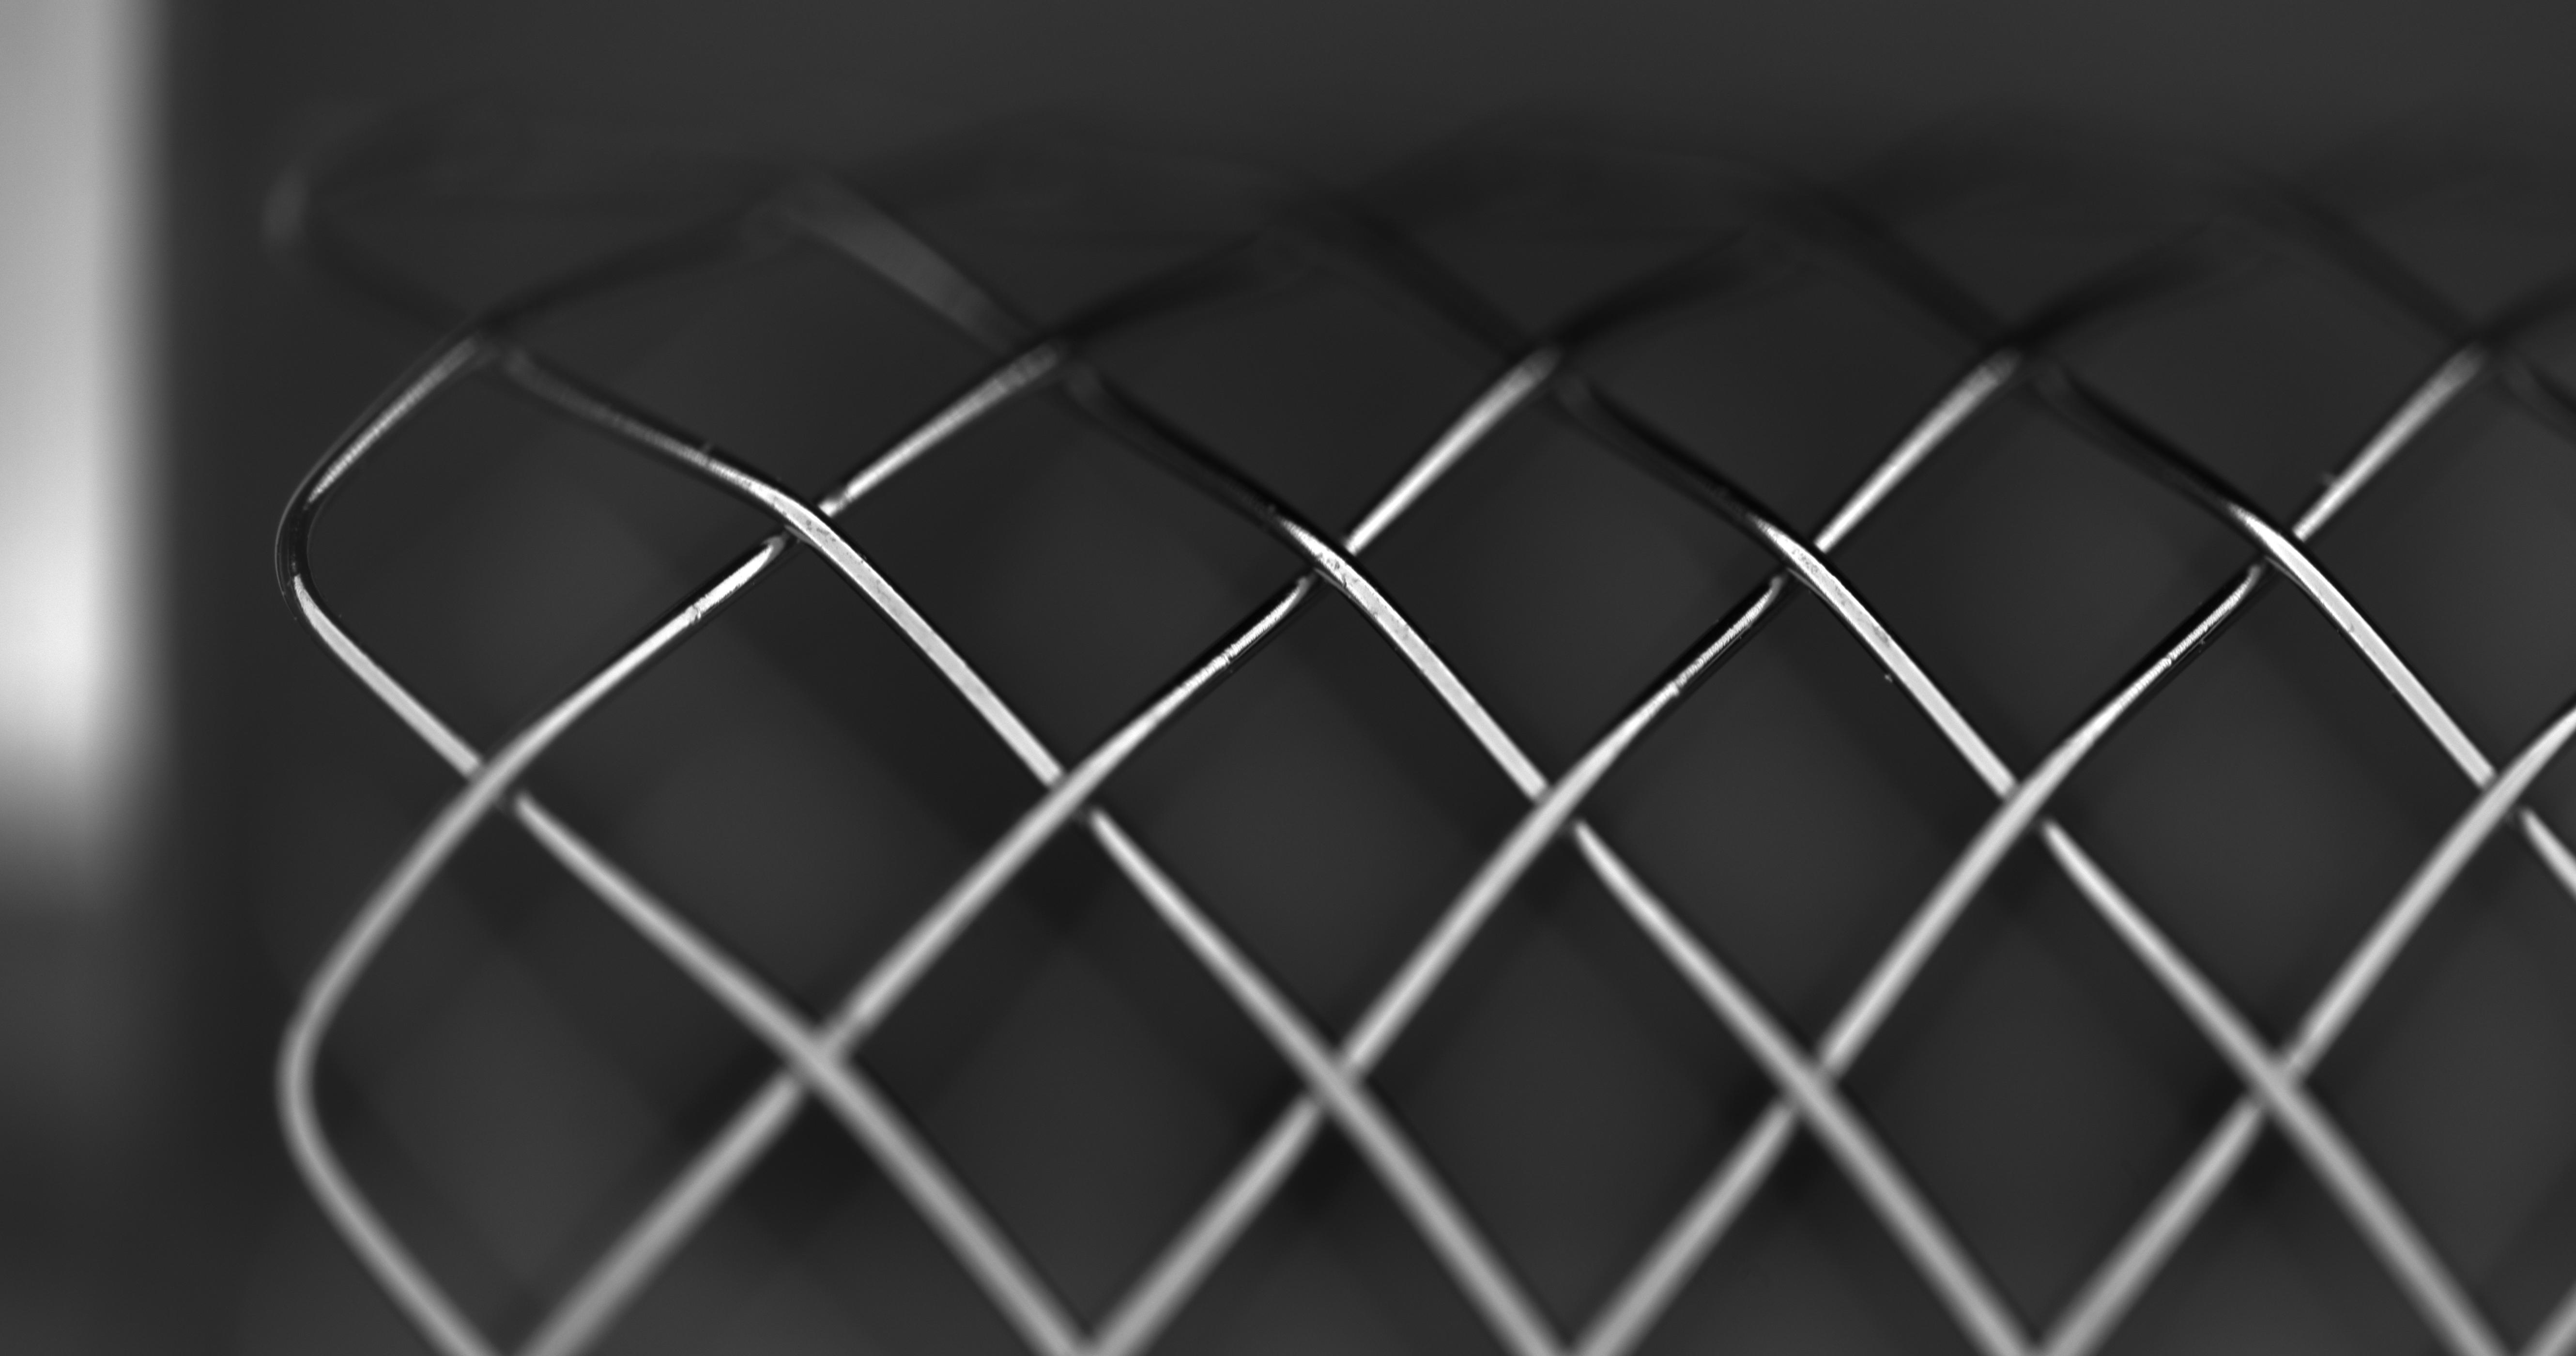
\includegraphics[height=2.4cm]{Bilder/Augmentation/mlr.jpg}
            
\includegraphics[height=2.4cm]{Bilder/Augmentation/mtb.jpg}
            
\includegraphics[height=2.4cm]{Bilder/Augmentation/mtlr.jpg}
            \caption{gespiegelte Aufnahmen. \scriptsize{Quelle: Yves Seburger}}
        \end{figure} 
        \item Rotation:
        \begin{figure}
            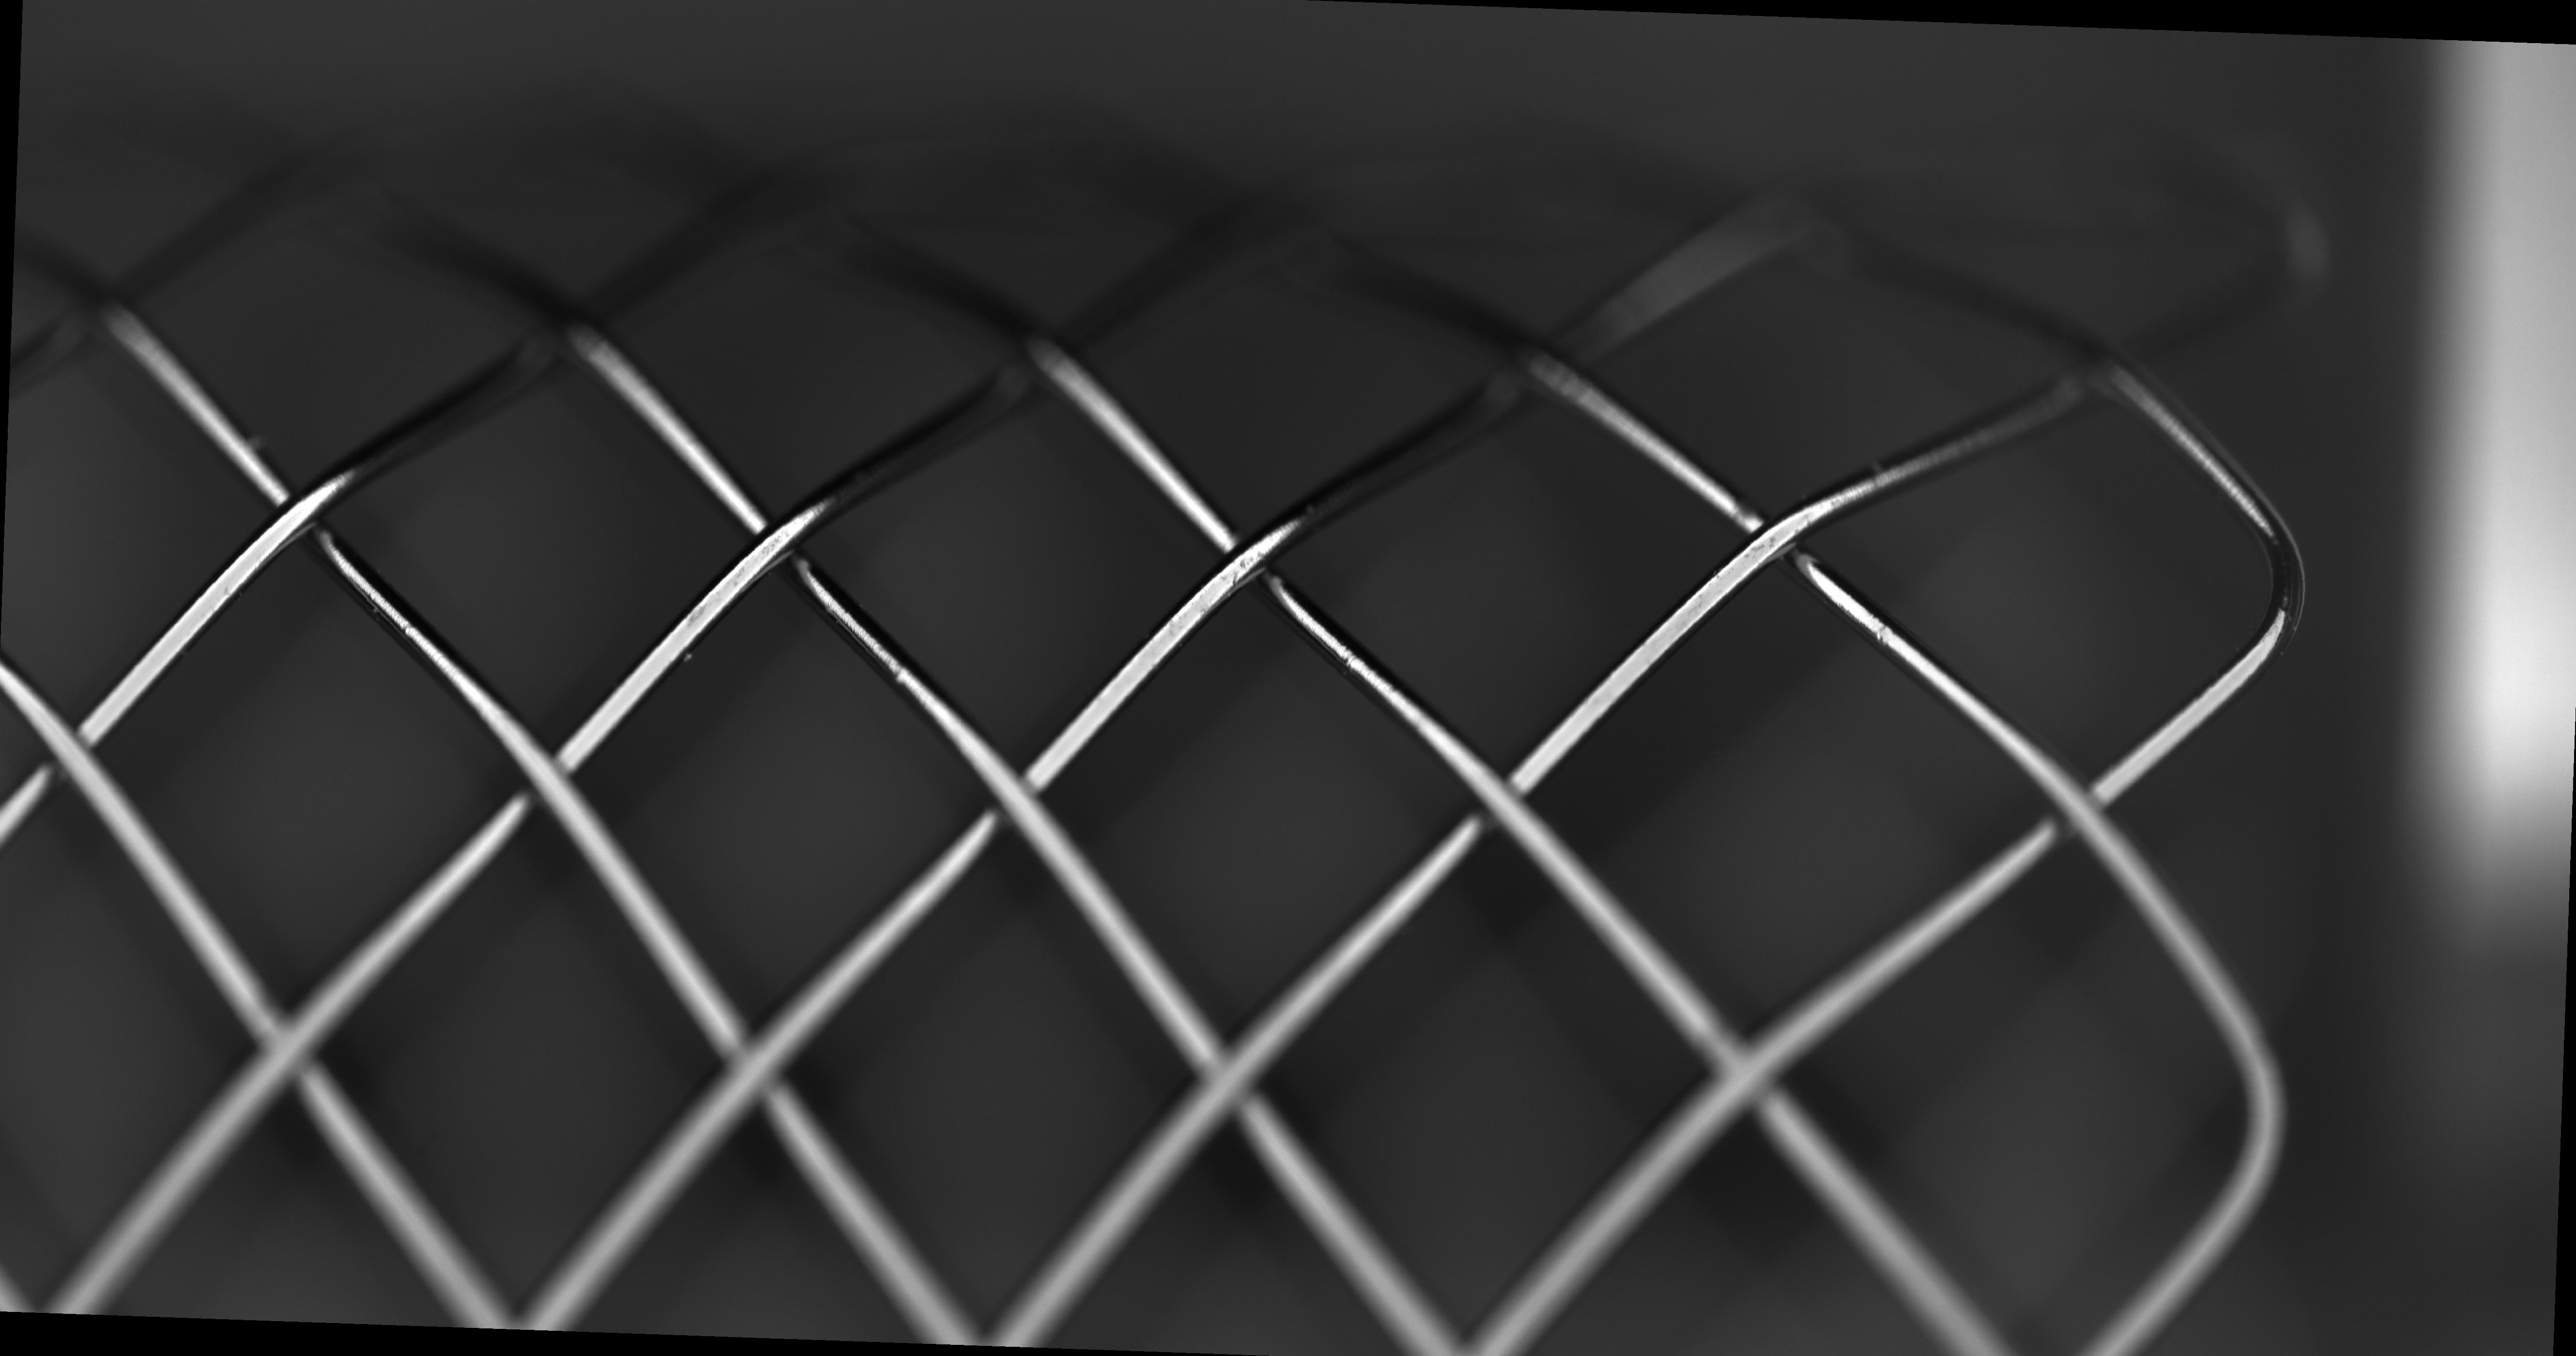
\includegraphics[height=2.8cm]{Bilder/Augmentation/-2grad.jpg}
            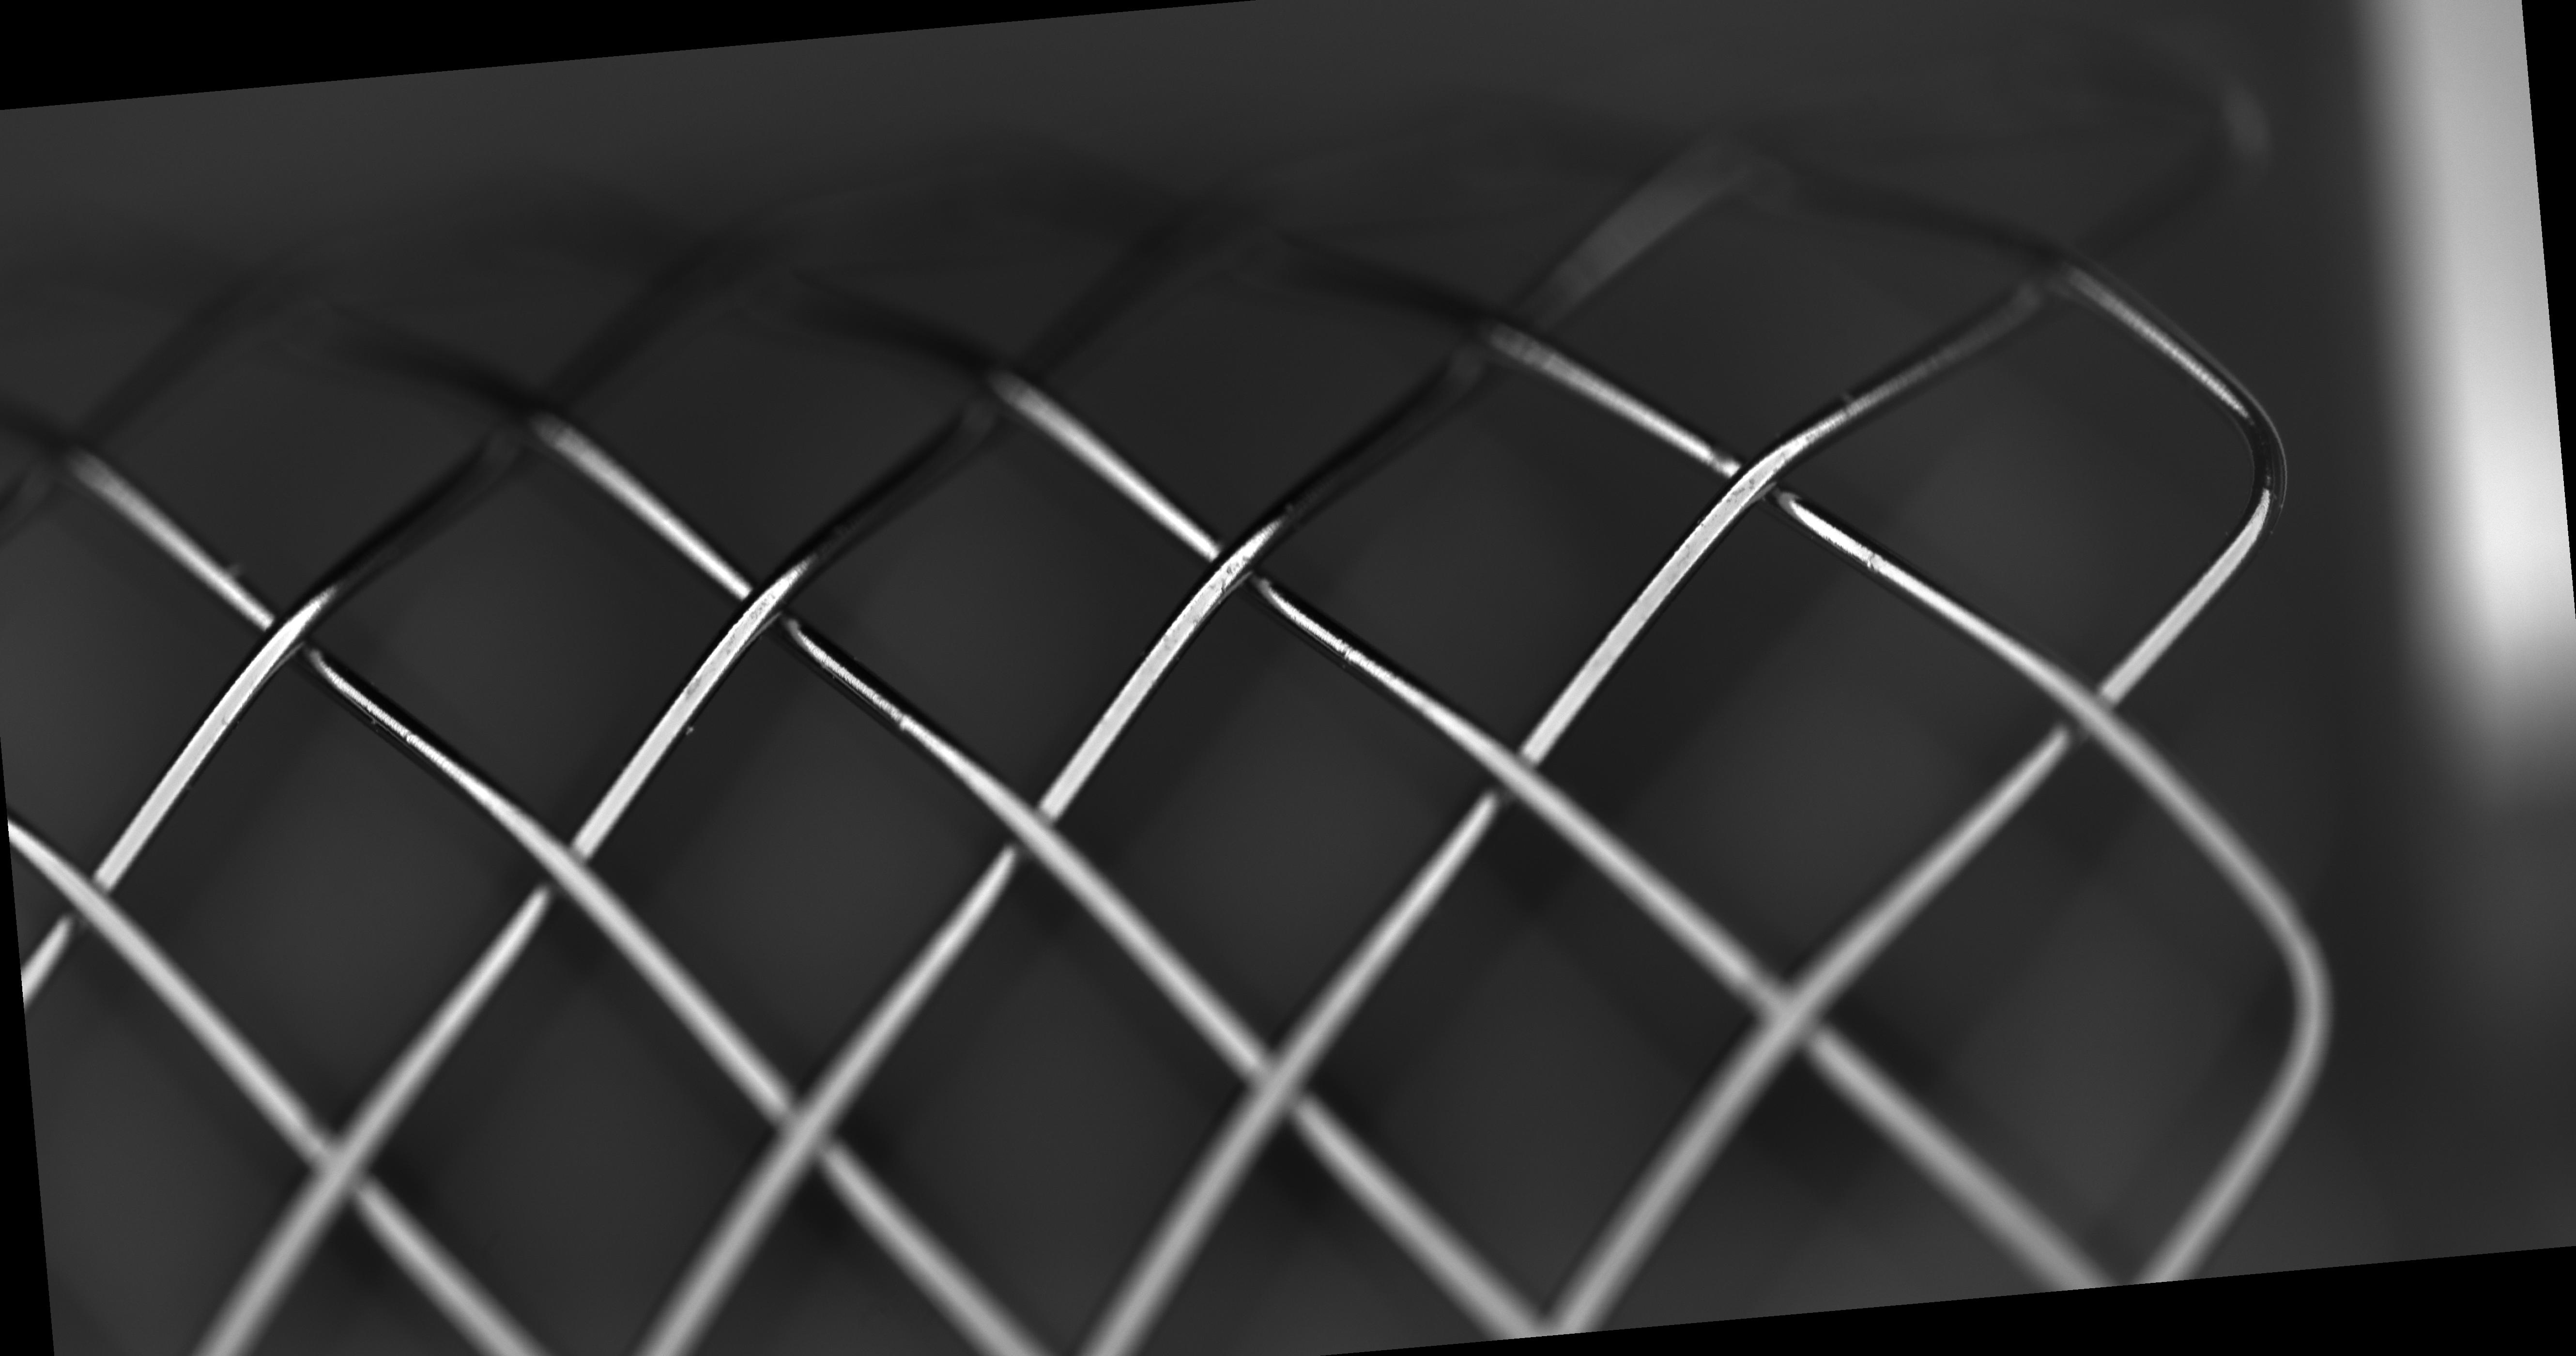
\includegraphics[height=2.8cm]{Bilder/Augmentation/5grad.jpg}
            \caption{rotierte Aufnahmen. \scriptsize{Quelle: Yves Seburger}}
        \end{figure}
        \item Weichzeichnen:
        \begin{figure}
            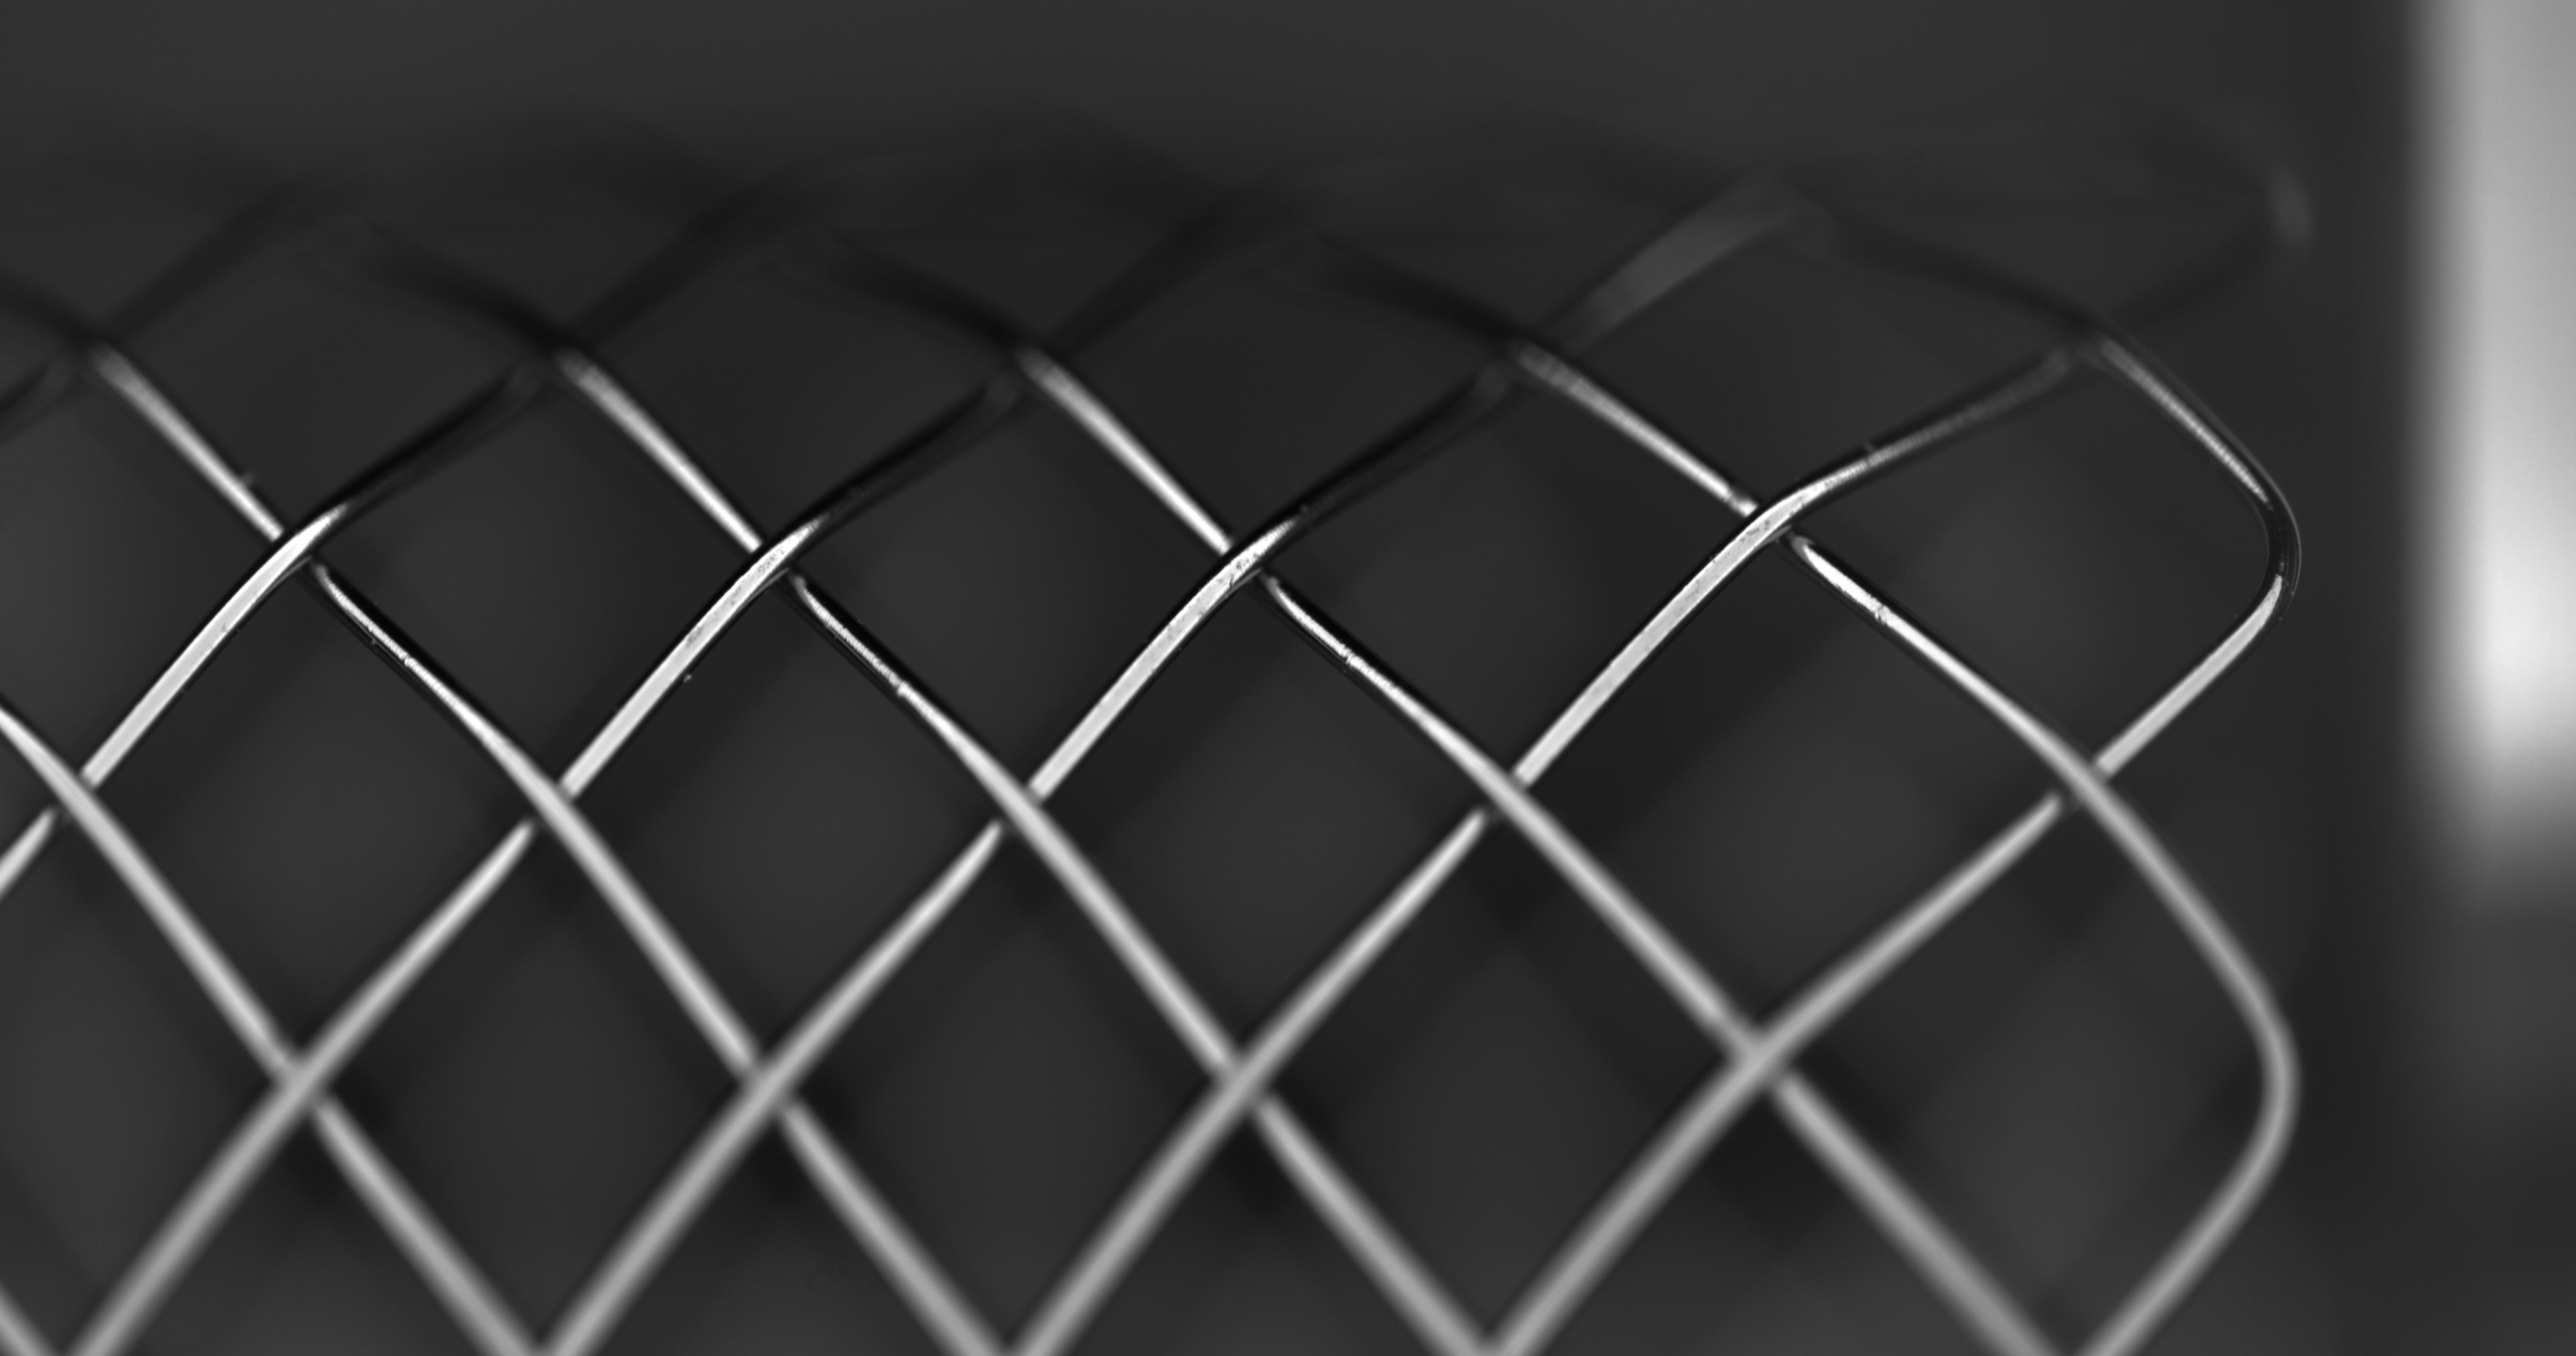
\includegraphics[height=5cm]{Bilder/Augmentation/gauss.jpg}
            \caption{weichgezeichnete Aufnahme. \scriptsize{Quelle: Yves Seburger}}
        \end{figure} 
        \item Kontrastveränderung:
        \begin{figure}
            \includegraphics[height=5cm]{Bilder/Augmentation/kontraständerung.jpg}
            \caption{kontrastveränderte Aufnahme. \scriptsize{Quelle: Yves Seburger}}
        \end{figure} 
        \item Verzerrung:
        \begin{figure}
            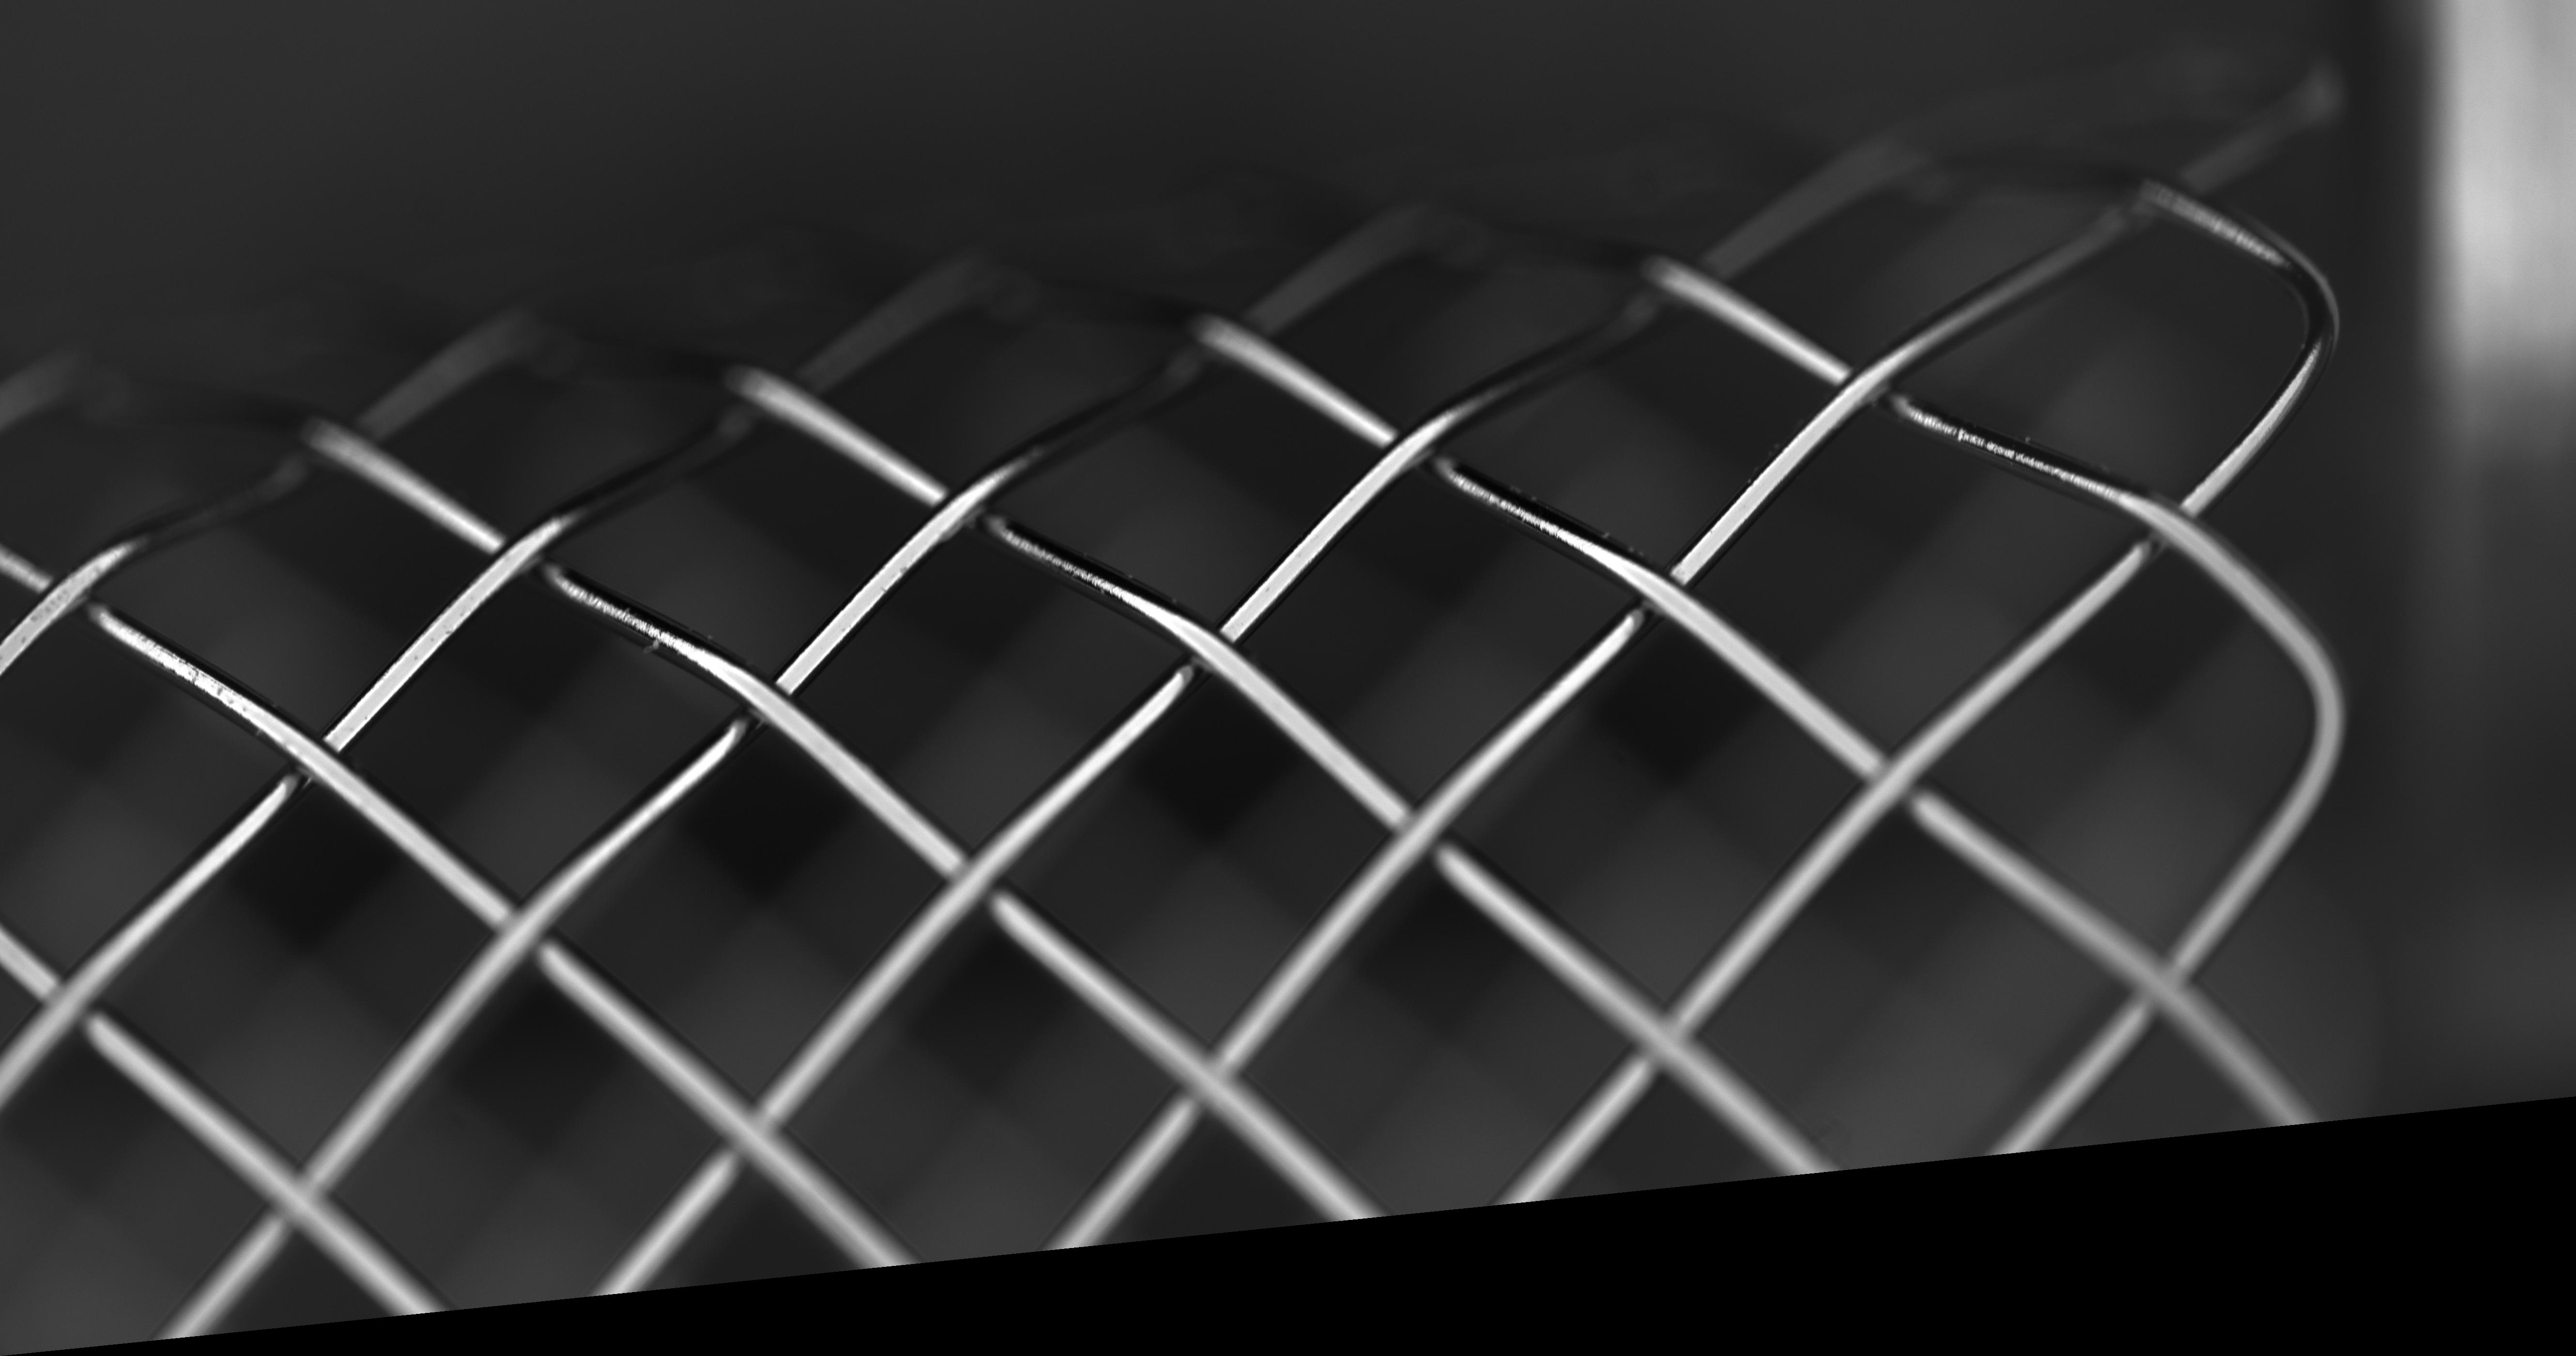
\includegraphics[height=5cm]{Bilder/Augmentation/verzerrung.jpg}
            \caption{verzerrte Aufnahme. \scriptsize{Quelle: Yves Seburger}}
        \end{figure} 
    \end{itemize}
    \item UNET
    \begin{figure}
        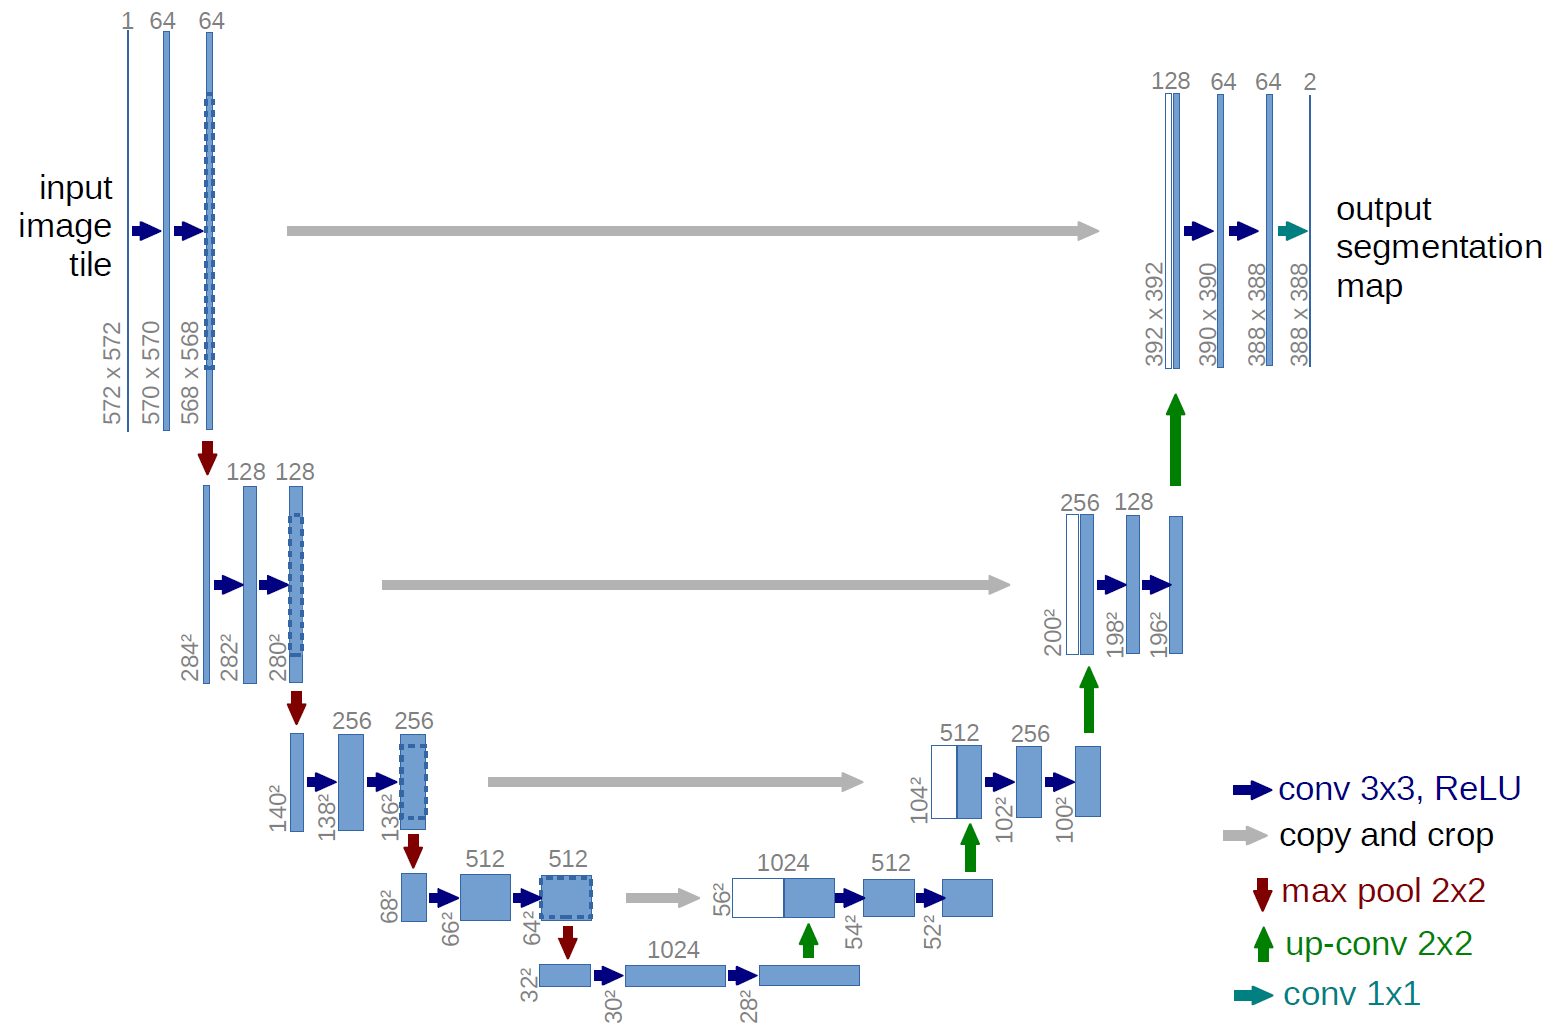
\includegraphics[width=0.8\linewidth]{Bilder/UNET_transparent.png}
        \caption{rotierte Aufnahmen. Quelle: \href{https://www.researchgate.net/profile/Blaz-Meden/publication/327635322/figure/fig2/AS:672158246252545@1537266422125/Illustration-of-the-training-data-The-top-row-shows-sample-images-from-the-CASIA.ppm}{Research Gate}}
    \end{figure}
    \item Half-UNET
    \begin{figure}
        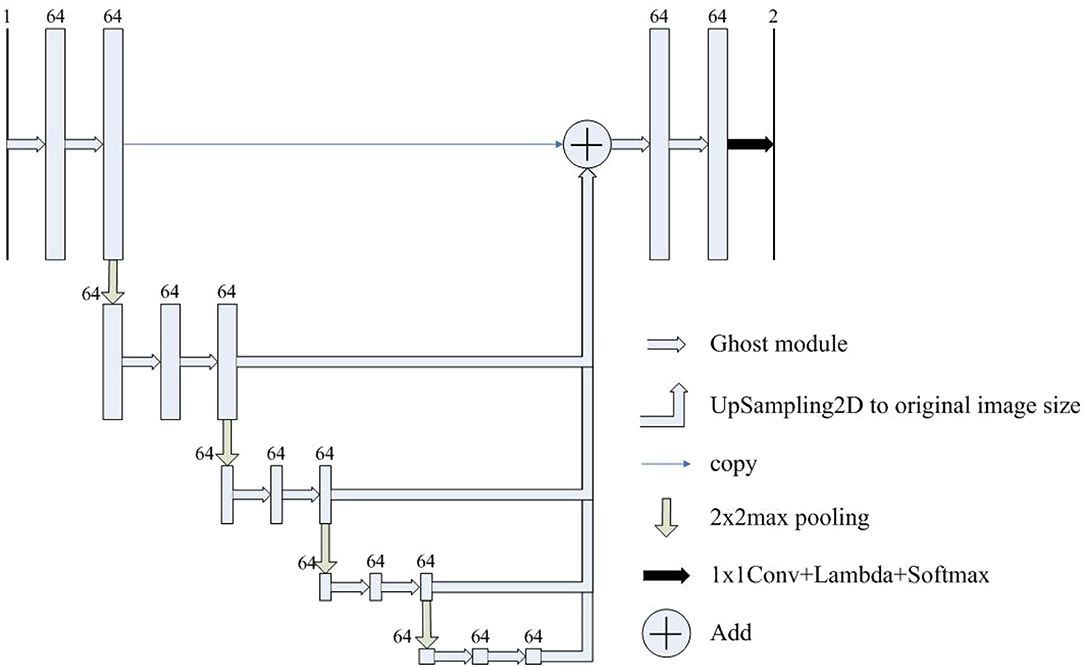
\includegraphics[width=0.8\linewidth]{Bilder/halfUNET.png}
        \caption{rotierte Aufnahmen. Quelle: \href{https://www.researchgate.net/publication/361186968/figure/fig3/AS:11431281182545975@1692382952577/The-architecture-of-Half-UNet-The-input-image-size-is-detailed-in-Table-2-The-numbers.tif}{Research Gate}}
    \end{figure}
    \end{itemize}
\end{frame}

\section{Resultate}
\begin{frame}[allowframebreaks]
\frametitle{Resultate}
\begin{itemize}
    \item verschiedene Trainingssets:
    \begin{figure}
        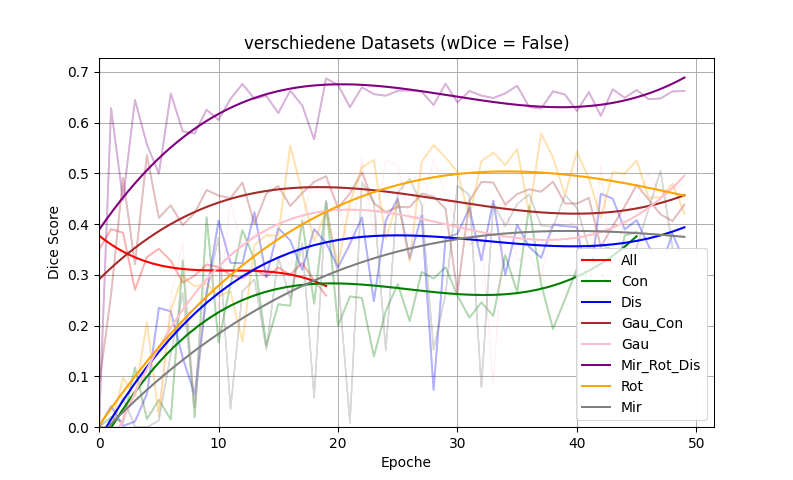
\includegraphics[width=0.85\linewidth]{Bilder/alle_Sets_false_trans.png}
        \caption{Dice-Scores für alle Datasets. \scriptsize{Quelle: Yves Seburger}}
    \end{figure}
    \framebreak
    \item Dice-Score vs. gewichteter Dice-Score
    \begin{figure}
        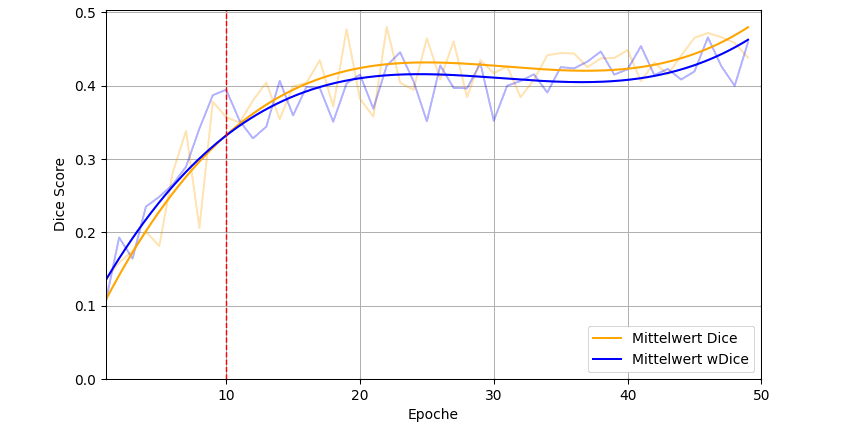
\includegraphics[width=0.95\linewidth]{Bilder/alle_Sets_true_vs_false.png}
        \caption{gemittelte Dice-Scores für alle Datasets. \scriptsize{Quelle: Yves Seburger}}
    \end{figure}
    \item UNET vs. HalfUNET
    \begin{figure}
        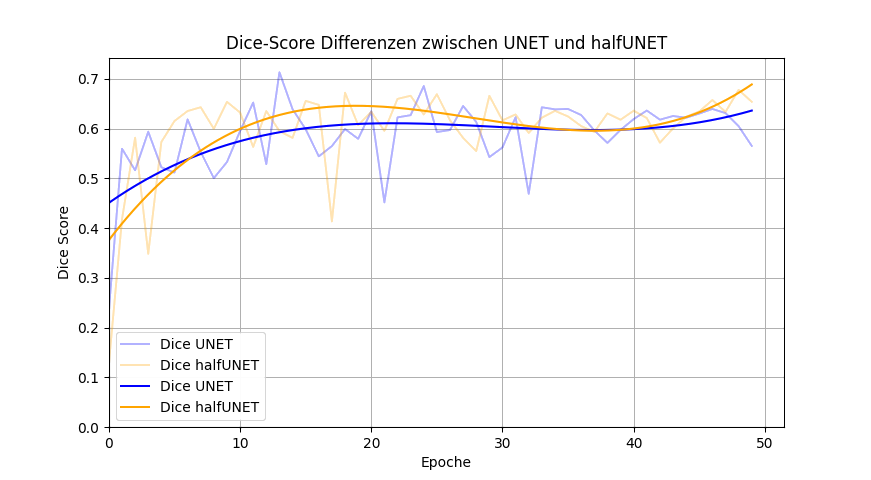
\includegraphics[width=0.85\linewidth]{Bilder/UNET_vs_halfUNET.png}
        \caption{UNET und HalfUNET im Vergleich. \scriptsize{Quelle: Yves Seburger}}
    \end{figure}
    HalfUNET \raisebox{0.5ex}{\texttildelow}$2,5 \times$ schneller, bei fast gleichem Resultat.
    \item Endresultat
    \begin{figure}
        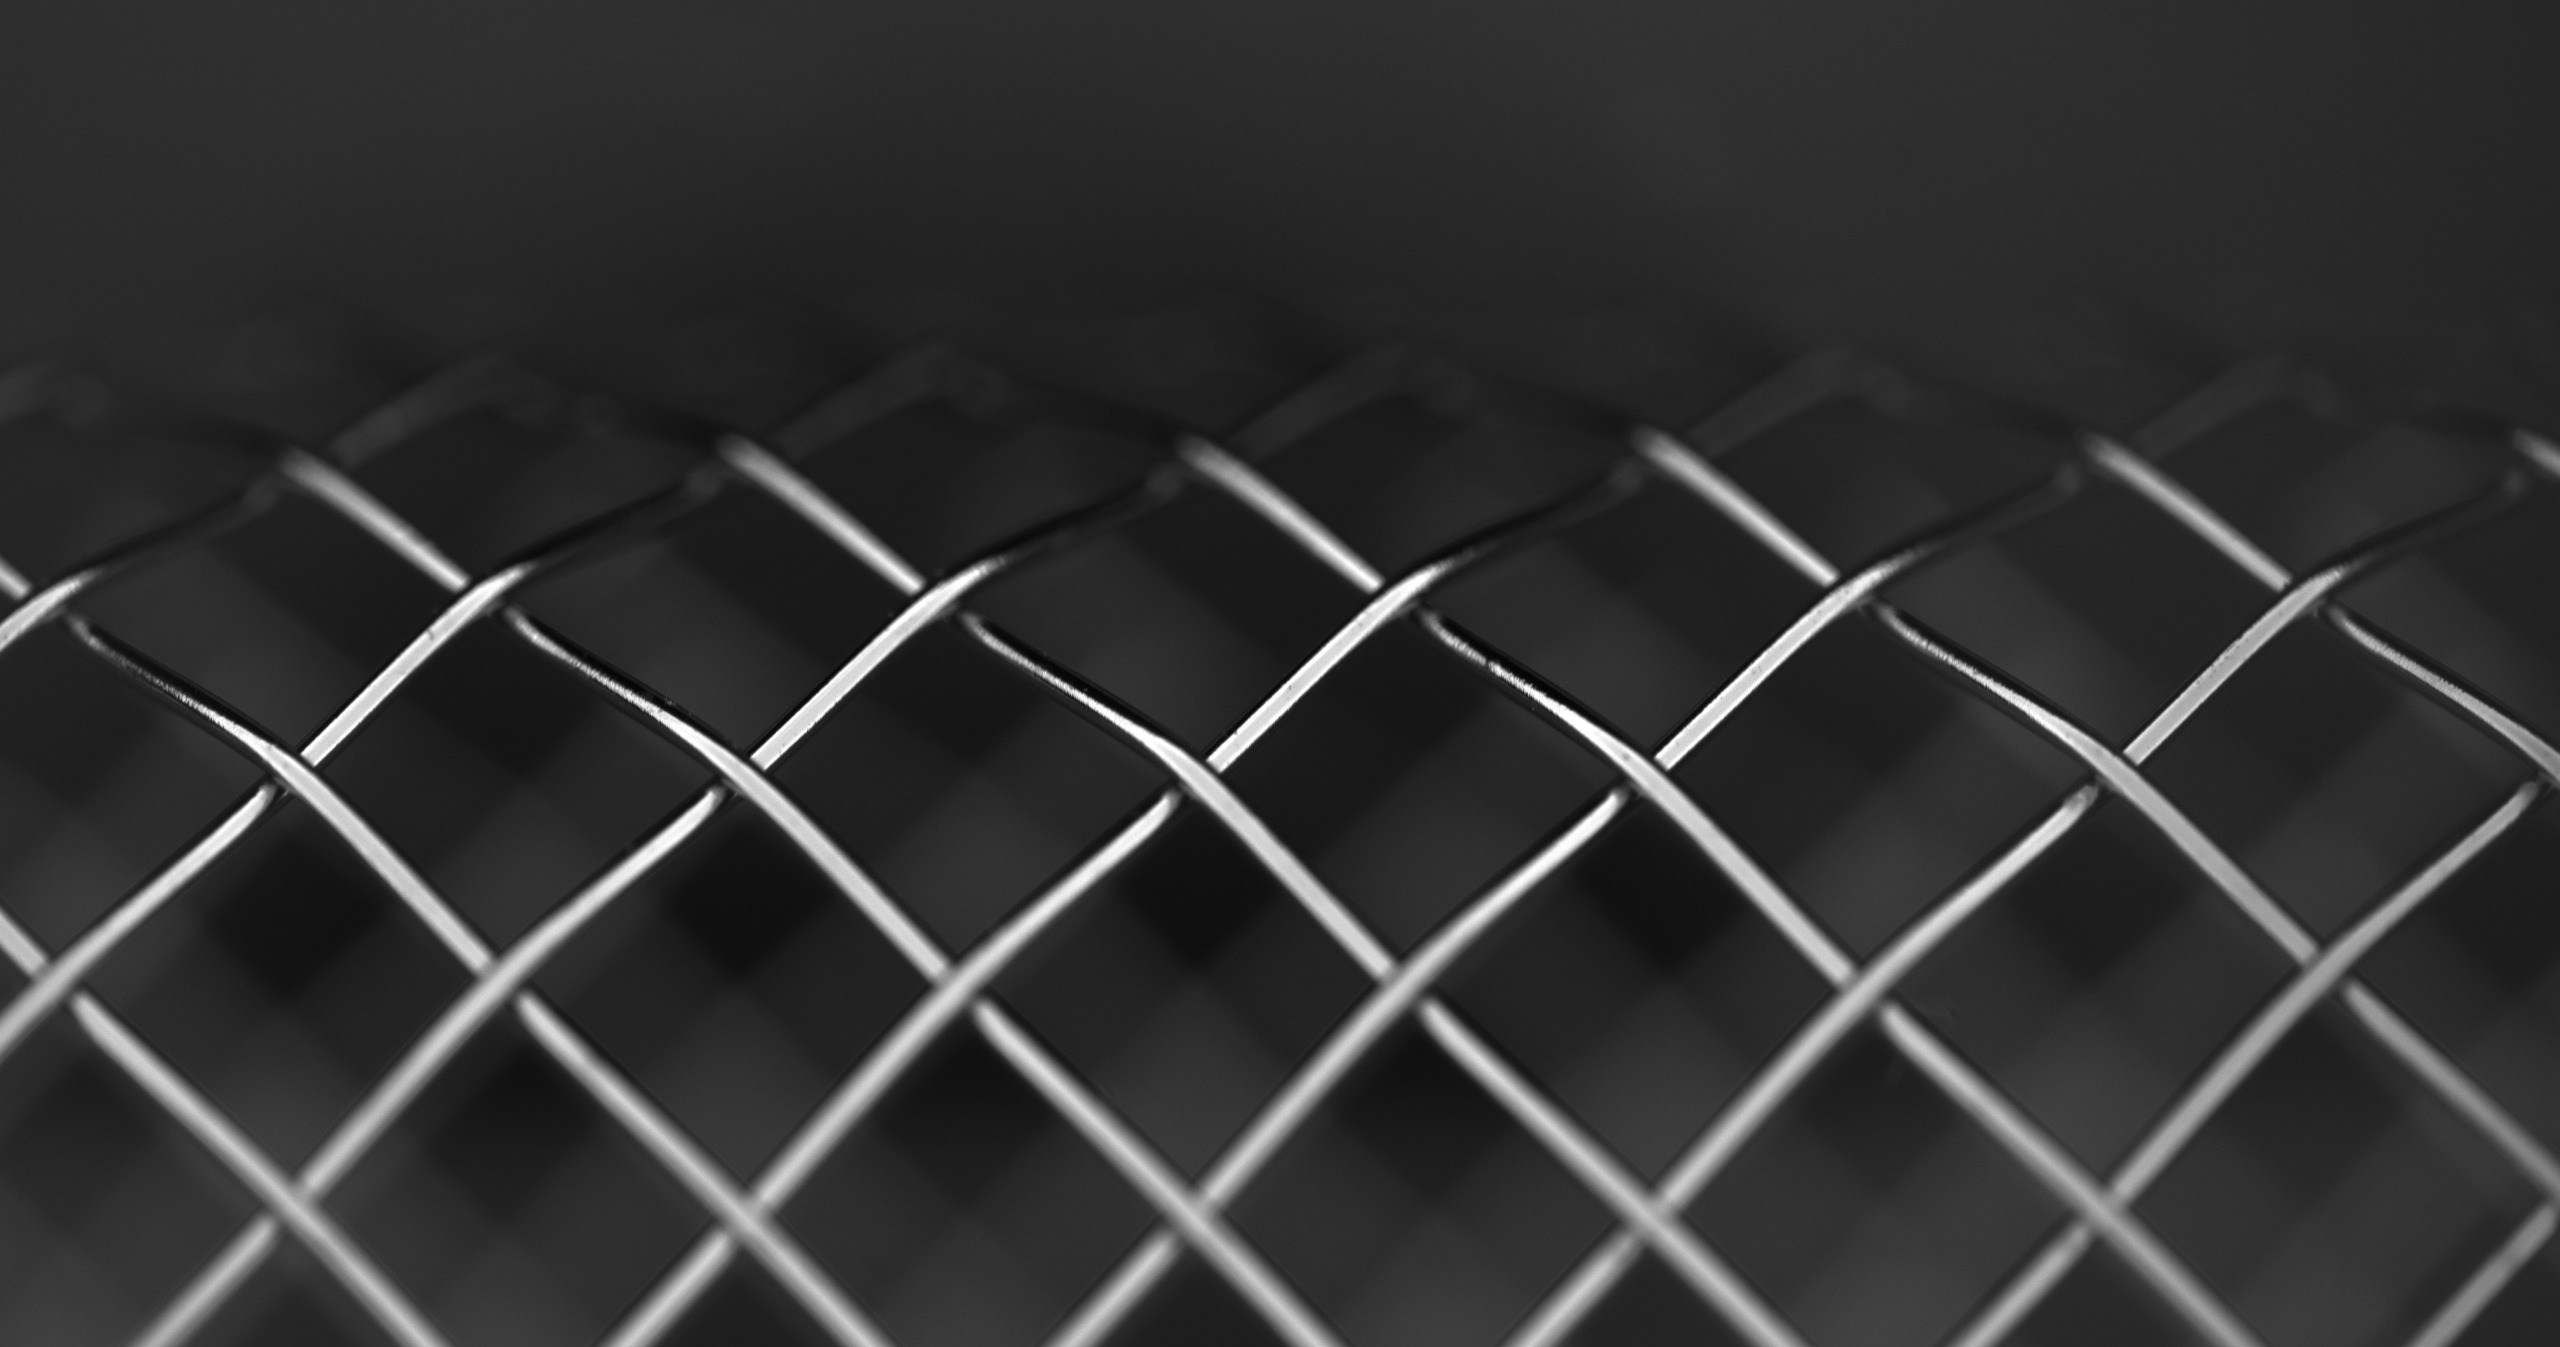
\includegraphics[width=0.9\linewidth]{Bilder/Original.jpeg}
        \caption{Originalbild. \scriptsize{Quelle: Yves Seburger}}
    \end{figure}
    \begin{figure}
        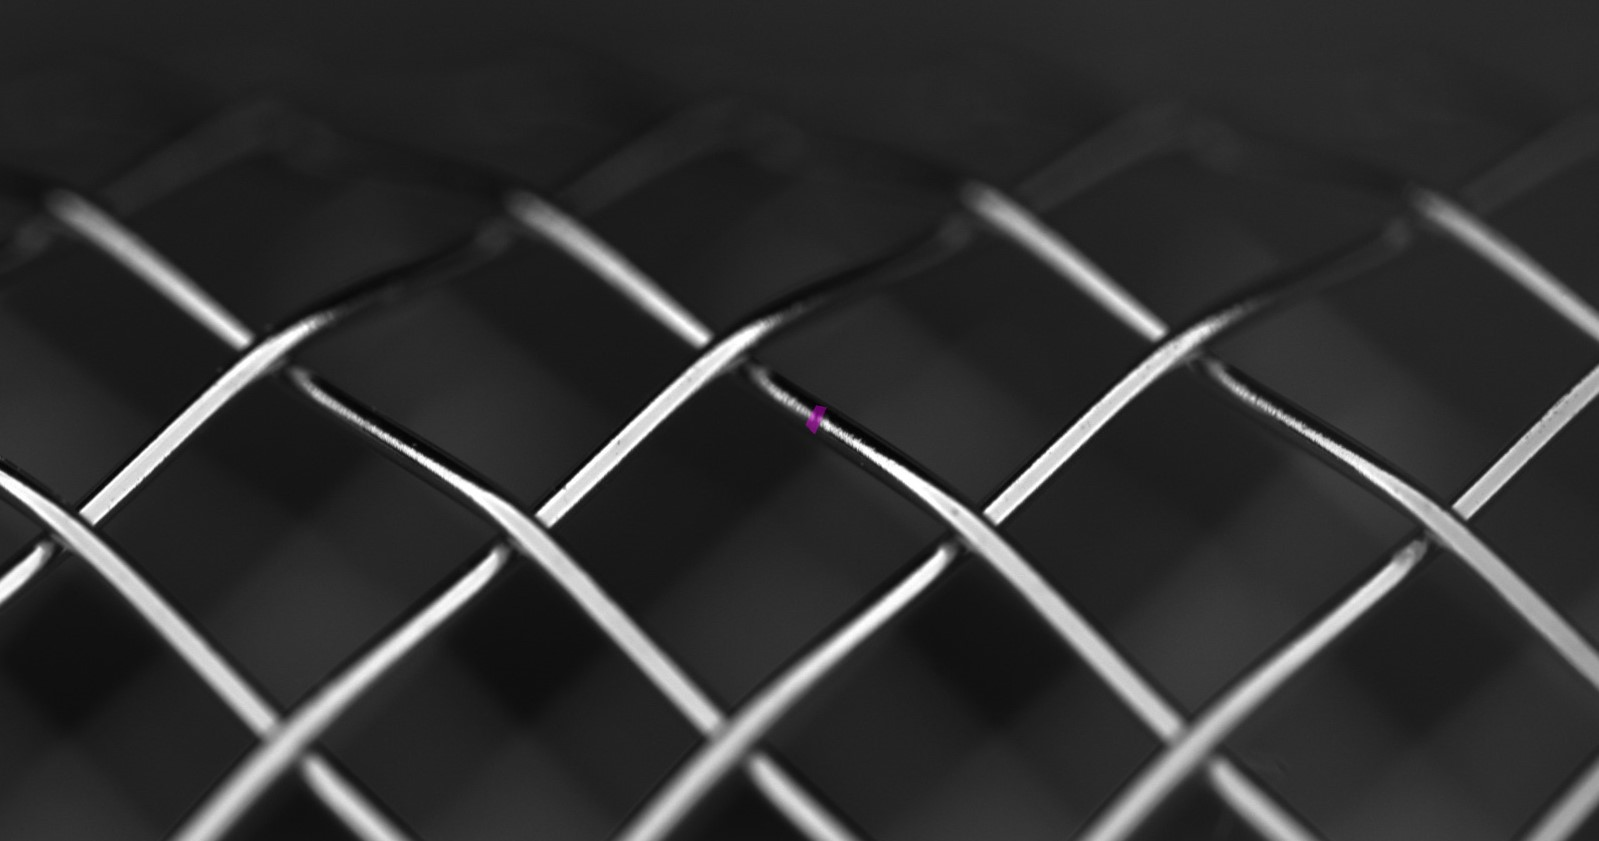
\includegraphics[width=0.95\linewidth]{Bilder/Original_und_Maske.jpeg}
        \caption{Originalbild mit überlagerter Maske. \scriptsize{Quelle: Yves Seburger}}
    \end{figure}
    \begin{figure}
        
\includegraphics[width=0.95\linewidth]{Bilder/Prediction_und_Maske.jpeg}
        \caption{Resultat der Prediction zur Visualisierung. \newline Dice-Score = \raisebox{0.5ex}{\texttildelow}0.77. \scriptsize{Quelle: Yves Seburger}}
    \end{figure}
\end{itemize}
\end{frame}

\section{Fazit und Ausblick}
\begin{frame}
\frametitle{Fazit und Ausblick}
\begin{itemize}
    \item Erweiterung der Aufnahmen
    \item Tests mit veränderlichem $\alpha$. \\
    \small{(Bisher nur linearer Anstieg, bis zur 10ten Epoche.)}
    \begin{itemize}
        \item Logarithmisch
        \item Exponentiell
        \item veränderliche End-Epochen für die Veränderung von $\alpha$
    \end{itemize}
    \item Qualität der Resultate
    \item Nutzung anderer Trainingssets (Autos, Vögel, etc.)
\end{itemize}
\end{frame}

\section{Fragen und Danksagung}
\begin{frame}[allowframebreaks]
    \frametitle{Fragen und Danksagung}    
    \begin{figure}
        \includegraphics[width=0.45\linewidth]{Bilder/Happy Stent.png}
        \caption{Fragen? \scriptsize{Quelle: Yves Seburger}}
    \end{figure}
    \framebreak
    Danke an:
    \begin{itemize}
        \item Prof. Dr. rer. nat. Martin Böhm
        \item Dipl.-Ing. Viktor Truderung
        \item Thomas Zimmermann M.Sc.
        \item Dipl.-Ing. (FH) Alexander Jäger
        \item Nina Schmitzer B.Eng.
        \item Dipl.-Ing. (FH) Raymond Seburger
        \item Lea Seburger
    \end{itemize} 
\end{frame}

\end{document}
